% =====================================================================================================
%  Radiology: Artificial Intelligence -- Original Research
%  RSNA supplies a Word template only; this file reproduces the journal's required structure
%  (title page, structured abstract <=250 words, summary statement, <=3 key points, abbreviations,
%  Introduction / Materials and Methods / Results / Discussion, <=3,000 words main text, tables, figure
%  legends, supplement with the CLAIM 2024 checklist). Every number is read from a result JSON written by
%  slurm/reproduce_feasibility.sh; see docs/FEASIBILITY_REPRODUCE.md. Nothing here is typed from memory.
% =====================================================================================================
\documentclass[11pt,letterpaper]{article}
\usepackage[margin=1in]{geometry}
\usepackage{setspace}\doublespacing
\usepackage{times}
\usepackage{graphicx,booktabs,array,amsmath,amssymb,xcolor,microtype,lineno}
\usepackage[labelfont=bf,font=small]{caption}
\usepackage[numbers,sort&compress]{natbib}
\usepackage[hidelinks]{hyperref}
%\linenumbers
\graphicspath{{figures/}}
\newcommand{\ci}[2]{[#1, #2]}

\begin{document}

{\Large\bfseries Graveyard: material cut from \emph{Naming Vertebrae Without an Anchor}}

\medskip\noindent This document holds everything removed from the manuscript's main text. None of it was discarded and none of it is required to read the paper, which is self-contained and does not cite this file. It is kept because the negative results in it are real results: four long-tail remedies that measured as doing nothing, an evaluation leak and what it was worth, a style filter that destroyed the anatomy it was applied to, and a transition-role head that lost. Where a number here disagrees with the paper, the paper's generated tables are authoritative and this file records what was written at the time.

\tableofcontents
\clearpage



\subsection*{S4. How this was arrived at, and what did not work}
The path to the result above was not straight, and the turns are recorded here rather than in the Results, where they would obscure the argument. Two of them are corrections to this work's own earlier figures; the rest are interventions that were tried and did not help. They are reported because a reader deciding whether to repeat any of them should know they have been run.

\subsubsection*{Withdrawal: the sweep arms scored spines the namer was trained on}
An audit of every sweep arm against the bank the namer was fitted on found a train/test leak in all of them. The namer is \texttt{model\_r18\_ce\_v3}, trained from \texttt{allspine\_v3\_fov96\_ctx}, which carries a patient-grouped train/val split. Of the 801 CT spines scored by the main arm and by the entire overlap ladder, 681 lie in that bank's train split, and of the 38 anomalous spines that carry the central claim, 30 do. Of the 170 real radiographs, 145 do; of the 76 VerSe spines, 64.

The Mendeley arm fails differently and just as completely. None of its 584 case identifiers appears in the bank, but 500 of them are re-encodings of BUU films---the filenames are BUU identifiers---and 417 of those originals are in the train split; its ordinary/unknown class split is exactly the duplicate/non-duplicate split, so the nominally ordinary group of 500 is 83\,\% pixel-duplicates of training films. Its levels are in any case named by counting upward from the most caudal body taken to be the sacrum, and a ground truth made by counting cannot test a system whose claim is that it replaces counting; no film carrying a sixth lumbar vertebra could be labelled correctly within it. That arm is discarded rather than re-run.

Nothing in the pipeline objected, because a sweep arm reads a render directory and a render directory does not record what a bank did with it. The tool now takes a \texttt{-{}-holdout-bank} argument and refuses to run without it, excluding any spine with a crop in that bank's train split, with an explicit override that writes its own use into the output record. Every sweep figure in the sections that follow is therefore withdrawn pending re-measurement on what survives the filter: 120 CT spines of which 8 are anomalous, 25 real radiographs, and 12 VerSe spines. Wide intervals on a true holdout are worth more than tight intervals on a memory test.

\subsubsection*{The size of the leak, measured inside a single run}
Comparing the contaminated arms against the fresh held-out arms would confound the leak with run-to-run variation, which at $n=120$ is worth roughly two points of chain completion. Splitting one run instead---same code, same seed, same random stream---by whether each spine lay in the namer's train split isolates the leak exactly.

The result is that the leak inflated the baseline rather than the treatment. On real films at two vertebrae, naming from the frame's own pixels falls from 82.4\,\% to 73.5\,\% when the trained-on spines are removed, and at three vertebrae from 92.3\,\% to 87.5\,\%; on VerSe at four vertebrae it falls from 48.1\,\% to 37.5\,\%. Naming the same frames through the sweep moves by between $-4$ and $+2$ points, with both signs, which is noise. Naming a frame from its own pixels is precisely the task that memorising a patient's vertebrae assists; naming it through the sweep is dominated by the chain and the correlation match, neither of which is learned. The quantity this paper is about---the improvement from placing a landmark-free frame on the sweep---is therefore larger on clean data than on contaminated data: on real films at two vertebrae it rises from $+12.2$ to $+18.4$ points, at three vertebrae from $+5.7$ to $+12.5$, and on VerSe at three vertebrae from $+66.7$ to $+77.3$. That is a fortunate shape for the error to have taken and is not offered as a defence of it; the absolute single-frame figures previously reported were wrong by five to eleven points.

\subsubsection*{Four encoders on one test set}
Accuracy read from each bank's own result file is not comparable across banks, which carry different validation splits, sources and class balances; by that reading bank v7 appeared six points below v6. Admitting only cases in the validation split of every bank and the training split of none gives 2,927 patients and 16,392 crops on which all four encoders name the same pixels. Bank v7 trained with logit adjustment is then the strongest model at 80.85\,\% exact, against 79.01\,\% for v6, 78.76\,\% for v2 and 77.14\,\% for v7 under cross-entropy: correcting the comparison reverses its sign.

At the sixth lumbar vertebra, accuracy rises from 67.4\,\% under v6 to 73.5\,\% under v7, a gain of 6.1 points on 105 held-out patients, with intervals of [59.0, 74.8] and [65.4, 80.3] that overlap. The result is suggestive rather than settled, but every earlier intervention aimed at this class measured as nothing at all, and this one did not. At the thirteenth thoracic vertebra all four models score zero on twelve patients, so the sixty-five real-film examples bought nothing. The test set requires membership of all three banks and therefore contains no FluoroCap images, which makes it a measure of whether real-film examples improve naming on the rendered distribution: for the sixth lumbar vertebra they transfer, and for the thirteenth thoracic they do not.

\subsubsection*{A label-preservation gate that exited without running}
The film-style adapter was applied to the CT renders to make them resemble photographed radiographs, and a gate was written to ask whether it had altered bone rather than only texture: the same encoder names the original and the filtered crop of one vertebra, and disagreement localises damage. The gate joined the two banks on case and level after stripping a \texttt{\_film} suffix from the case identifier. The suffix is a style seed, \texttt{\_s0}, and \texttt{\_film} sits on the source field instead; no pair matched, the gate raised, and the merge consuming the filtered crops proceeded regardless.

With the key corrected the gate reports 86.5\,\% agreement on \texttt{ctsp\_drr} renders and 73.3\,\% on VerSe renders, against 32.7\,\% on \texttt{physics\_drr} and 36.7\,\% on \texttt{physics\_rare}---which together are 79\,\% of the filtered bank and the source of most rare-variant examples. Encoder accuracy falls from 72.7\,\% on the original crops to 40.0\,\% on the filtered ones, and 7,066 of 9,443 renders flip more than a fifth of their bodies. The adapter damaged those renders rather than restyling them.

The harm is bounded: no result file names the bank this produced, so nothing downstream was trained on it. The gate's design was sound and only its join key was wrong, which is the more instructive failure---a check that fails open produces the paperwork of having looked. A zero-match exit now prints both key sets and states that the gate did not run.

\subsubsection*{Bank v7: the first real-film examples of the failing classes}
FluoroCap's decoded panels entered a training bank for the first time, and the count that matters is distinct patients carrying each variant class rather than crops. Bank v5 held 168 patients with a sixth lumbar vertebra and thirteen with a thirteenth thoracic, every one of them a CT render. Bank v7 holds 213 and 73, of which FluoroCap contributed 83 and 65 respectively---the first photographs of either variant anywhere in the corpus. VinDr contributed a further 43,244 crops across L1--L5 and the sacrum. Panels were rotated upright using the orientation network's own recorded call before any crop was cut, because the stored boxes are in the rotated frame and thirty-nine of the first four hundred panels required a half turn.

This does not by itself repair the L6 figure: 213 patients against roughly 11,000 at L4 remains a fifty-fold imbalance, and the two interventions designed for that imbalance were both measured as doing nothing. What it makes possible for the first time is the question of whether a real six-lumbar spine teaches something a rendered one does not, which no previous experiment could ask.

\subsubsection*{Four remedies tested, three refuted}
Each remedy was trained on the same recipe and scored by the same evaluator against the v2 baseline of 91.8\% ordinary and 66.0\% anomalous on interior windows. Domain randomisation with the fitted film-noise model applied to every training render (bank v2fm, 40 epochs) gave 91.7\% \ci{89.2}{94.1} ordinary and 59.6\% \ci{31.1}{90.6} anomalous: no gain, and the anomalous interval spans the baseline. Pretraining on renders alone and fine-tuning on real film---the SyntheX recipe, and the one theory of this project that most deserved a test---gave 89.1\% \ci{86.3}{91.6} ordinary and 40.4\% \ci{14.5}{69.2} anomalous, worse than training on the mixture directly, which is the arrangement already in use. Mixing renders and real film at full strength for the same eight epochs gave 88.2\% and 36.2\%. The synthetic-fraction sweep explains why the mixture is nonetheless right: holding real film fixed and raising the render fraction from none to half moved anomalous accuracy from 34.0\% to 53.2\% while ordinary accuracy fell 2 points, and holding renders fixed while cutting real film from all to a quarter cost 5 points of ordinary accuracy. Renders buy variant anatomy that the real collections do not contain; they do not buy the film domain, and no amount of them substitutes for real film. The two pseudolabel-admission rules complete the set. Admitting only the decodes whose placement reached a landmark gave 88.4\% \ci{85.6}{91.1} ordinary and 36.2\% \ci{11.1}{68.2} anomalous. Admitting them at a rate that falls with the predicted class's frequency, the CReST rule, gave 87.5\% \ci{84.5}{90.5} and 59.6\% \ci{30.4}{91.1}, on 952 of 63,869 eligible rows---the exponent that protects the rarest class starves the others. Neither reaches the baseline that admits no pseudolabel at all. A fifth intervention, aimed at the rare classes rather than at the pseudolabels, is the only one that moved a number: logit adjustment---shifting the logits by the log class prior during training so that the plain argmax is already the balanced argmax, rather than re-weighting samples \citep{menon2021}---gave 93.8\% \ci{91.4}{96.0} on ordinary interior windows against the baseline's 91.8\%, 99.7\% on cervical, and 96.2\% on held-out NHANES lumbar films, which is the best single-frame figure in this study. On anomalous spines it gave 59.6\% \ci{30.9}{90.0} against 66.0\% \ci{39.6}{87.2}---twelve films, which settles nothing. Repeated on the v6 bank, whose held-out set is 128 anomalous films, it gave 92.8\% \ci{90.1}{95.2} ordinary against 89.9\% \ci{87.1}{92.7}, cervical 99.5\%, and 47.0\% \ci{38.3}{55.9} anomalous against 49.9\% \ci{41.5}{58.9}. With a denominator five times larger the anomalous intervals still overlap across most of their range. Logit adjustment therefore buys about three points on ordinary spines and nothing on transitional ones, which is a properly powered null rather than an underpowered one, and it locates the rare-class problem somewhere other than the decision rule. A sixth was the second view. BUU photographs every study twice, and all 3,600 pairs were scored through one encoder and one head, so that lateral alone, anteroposterior alone and each fusion differ only in which posteriors enter one decode. The lateral film alone named 92.7\% \ci{92.0}{93.5} of vertebrae in a two-body window and 94.7\% \ci{94.0}{95.4} in a three-body one; the anteroposterior film alone named 46.5\% \ci{45.2}{47.8}. Three pooling rules were tried---the arithmetic mean of the two posteriors, their normalised product, and a mean weighted by each view's own confidence---and none beat the lateral alone (92.7, 92.7, 92.8 at two bodies), while at three bodies every rule lost (93.8, 93.1, 94.0 against 94.7). Repeating the arm with the v6 encoder gave the same verdict from the other side: lateral 91.7\% \ci{91.0}{92.5}, anteroposterior 40.6\% \ci{39.5}{41.8}, and fusions of 92.0, 92.2 and 91.9 at two bodies---half a point, well inside the interval---and 93.8, 93.8, 93.9 against 93.8 at three. Averaging a weak opinion into a strong one costs more than it adds. Because the encoder was trained overwhelmingly on lateral films, this refutes two-view fusion with this encoder rather than the idea; an anteroposterior-competent encoder is a separate experiment. The arm could not be split by spine class, because the per-study anomaly reading was not loaded into it. Four remedies, four refutations: on this problem, a pseudolabel whose names come from a decoder carrying the ordinary prior cannot be rescued by choosing which of them to believe, and the intervention that remains is a reader.

\subsubsection*{Why the larger bank lost, component by component}
Bank v5 is 2.4 times bank v2 and scores worse on the spines this study is about. The bank was rebuilt five ways on one recipe and one held-out set to find out which component did it (interior windows, film-cluster bootstrap). Bank v5 entire: 91.2\% \ci{88.8}{93.5} ordinary, 52.8\% \ci{29.0}{73.7} anomalous. Remove the decoder-named pseudolabels and ordinary falls 1.5 points to 89.7\% while anomalous rises 19 points to 71.9\% \ci{45.9}{90.5}. Remove the oblique renders instead: 90.0\% and 58.4\%. Remove the extra real-film sources instead: 88.7\% and 69.7\%. Remove all three and the bank collapses to 85.3\% and 38.2\%. The pseudolabels are therefore the component that trades anomalous accuracy for ordinary accuracy, and they trade it at about thirteen points of anomalous accuracy per point of ordinary. They are 30.0\% of the bank and 29.5\% of its lumbar training rows, and they were named by a decoder whose own prior is the ordinary alphabet; a spine that does not fit that alphabet is named as though it did, and the network learns the prior rather than the anatomy. This is the reason the deployed configuration is trained without them, and the reason the students' review (Discussion) is the intervention with the most to give.

\subsubsection*{Pseudolabel quality, measured against human names}
Matched geometrically to the 543 human-labelled NHANES films, the decoder's exact-tier names agreed on 96.3\% of cervical bodies on anchored films (n\,=\,970), 89.9\% of lumbar bodies on anchored films (n\,=\,258), and 100\% of lumbar bodies on unanchored films (n\,=\,1,064). Two earlier versions of this comparison reported 0.23\% and 40\%; the first zipped levels by list index while the human set names one more level than the decoder does, and the second keyed a patient's cervical and lumbar films by the same number, so that cervical pseudolabels were scored against lumbar human levels. The high agreement is on ordinary spines under a shared counting convention; it is not evidence that the pseudolabels are right on anomalous spines, which is where training on them cost twenty points. The anchoring gate kept 8,639 cervical and 1,448 lumbar NHANES films, 2,233 cervical and 2,898 lumbar VinDr films, and 203 laterals, and queued 11,323 films---6,147 NHANES lumbar films with no sacrum or rib zone in the decode among them---for annotation.

\subsubsection*{The film-noise model, fitted}
Renders sat outside the real films' quality band before any augmentation: median crop signal-to-noise ratio 327 against 164 on real film, noise 0.0029 against 0.0059. A first, guessed setting of the knobs overshot to noise 0.049 and SNR 20 and was discarded. The grid-fitted setting (photons 80,000--800,000; read noise 0.05--0.4; blur 0.1--0.4 px; scatter fraction 0.05--0.25) brought the render medians to 0.0068 sharpness (real 0.0078), 0.0073 noise (real 0.0059), and SNR 136 (real 164), inside the real p10--p90 band on three of four statistics; contrast (0.988 against 0.949) remained just outside (Fig.~S5). Every training render crop in the v2fm bank passed through that setting with a fresh random draw; real and validation crops were untouched.

\subsubsection*{The predicted mechanism is real and bounded (C3)}
Of 4,774 State-C errors in v2, 83.0\% were exactly one level (52.0\% one level too low, 31.0\% too high; Fig.~4); errors of half a level, i.e.\ a variant class confused with its neighbour, were a further 10.7\%. Of 2,003 errored windows, 899 (44.9\%) carried one coherent offset across every vertebra in the window---the $P(B\mid M_5)\approx P(B\setminus b_1\mid M_6)$ degeneracy exactly as described---while 514 were scattered. Coherent whole-window shifts were 8.3\% of all State-C windows.

\subsubsection*{CT-tuned thresholds collapse on film, and the decoder prefers variants only where it cannot see (C4)}
At thresholds fitted to 95\% specificity on CT renders, the template log-likelihood ratio fired on 100\%, 92.6\%, and 99.3\% of NHANES, VinDr, and AASCE films; the anchor-and-count disagreement on 0\%, 100\%, and 100\%; the expected-lumbar-count on 0\%, 97.1\%, and 100\%; and the count-versus-morphology divergence on 2.1\%, 33.0\%, and 99.3\%. The report predicted 50--65\% specificity; the collapse was total. The whole-spine template decoder behaved in the opposite way to the one we first reported. Of 10,274 VinDr films it named, it chose a variant template on 191 (1.9\%; 165 L6, 24 T13+L6, 2 T13), and 164 of the 191 (86\%) contained a sacrum in the decoder's placement; the variant rate was 9.0\% \ci{7.8}{10.4} on films with the sacrum in the decode against 0.32\% \ci{0.22}{0.46} without, rising with the number of detected bodies to 30--60\% at nine or more. Against a population prevalence of 4--9\% for a 25-presacral spine, most of those calls are false positives made where the junction was visible, not blind shifts. (An earlier analysis read the junction from the supervision tier that the pseudolabelling script itself clears on flagged films, which made ``flagged'' and ``junction absent'' one statement; an adversarial review caught it.)

\subsubsection*{The geometric substitutes do not transfer (Table~4, Fig.~6)}
On 3,456 ordinary lateral films the median Wigh index of the lowest body was 2.08 (interquartile range 1.77--2.46); 5.1\% fell in the report's ``normal L5'' band of 1.20--1.45, and 0\% on anteroposterior films (median 4.50). For six-lumbar spines (n\,=\,15) every index had an AUC whose interval crossed 0.5 except sacral slope, 0.73 \ci{0.61}{0.84}, with the six-lumbar median 29.4$^\circ$ against 36.2$^\circ$. For four-lumbar spines (n\,=\,129) the L5--S1 gap separated near-perfectly, AUC 0.99 \ci{0.99}{1.00} (median 0.14 versus 0.44 body heights), and the Wigh index of the lowest body reached 0.78 \ci{0.74}{0.82}. The criterion that is actually in the literature fared no better: the superior-to-inferior end-plate ratio had an ordinary median of 1.02, so the published rule of 1.37 or less fired on 99.9\% of ordinary lateral films, and as a continuous index it was at chance for six-lumbar spines (AUC 0.54 \ci{0.39}{0.68}). Sixty-seven percent of ordinary films had a sacral slope in the report's 30--50$^\circ$ band. The near-zero L5--S1 gap on four-lumbar films is the annotation schema, not anatomy: BUU's keypoints are fixed at five lumbar bodies and its authors state that on sacralisation the fifth set of corners lands on S1 \citep{buu2023}, so on those films the annotated ``L5''--``S1'' gap is the S1--S2 junction (Discussion). BUU does not, however, hide the anomaly: the authors' L4L6 sheet records it per study. The schema correction succeeded on every study it was designed for: the per-study resize fit (scale 0.84--1.17) had a residual of at most one pixel on all 15 six-lumbar films, so all 15 received an L6 box; the 129 sacralised studies received a transitional flag on L5; none was refused; and all 144 were marked ineligible for training so that no future bank repeats the contamination.

\subsubsection*{A sweep of overlapping frames replaces the CT (Fig.~7, Table~6)}
The limitation the interior-window result establishes is real and it is not a limitation of the network: it is a limitation of one exposure. Sweeping restores what one exposure cannot hold. Every arm below uses the field of a 9-inch image intensifier, about 14\,cm at the spine, which is what a mobile C-arm actually gives.

On all 801 abdominopelvic renders that reach the sacrum, with one body of overlap, the chain of vertebrae came out complete---no duplicated, missed or spurious node---on 94.1\% of spines from a mean of 2.4 frames, and the chain itself was named at 95.5\%. A limited-field frame of two vertebrae, named on its own pixels, was correct 70.7\% of the time; the same frame registered onto the sweep was correct 93.6\%, and the registration put it in the right place 96.4\% of the time. At three vertebrae the figures were 84.5\% alone and 94.0\% mapped; at four, 90.6\% and 95.1\%. The gain does not fall away on variant anatomy: on the 25 lumbosacral-variant spines a two-body frame went from 67.3\% to 85.7\%, and on the 11 thoracolumbar-variant spines from 50.0\% to 95.5\%.

\emph{Overlap is the knob, and it is free.} Holding the field and everything else fixed and varying only how far the C-arm moves between exposures, two-vertebra frames scored 86.6\% at half a body of overlap, 93.6\% at one, 95.1\% at two, 95.2\% at three and 93.2\% at four. The optimum is two bodies: below it the linker is working from partial bodies at the seam, and above it the extra exposures add links faster than they add evidence---chain completeness falls from 94.2\% at two bodies to 80.4\% at four. Field size, by contrast, barely moved the naming (94.9\%, 93.6\% and 93.5\% at two vertebrae for a collimated, a 9-inch and a 12-inch field) while chain completeness rose with it (92.5\%, 94.1\%, 96.5\%), because a wider field needs fewer links.

\emph{A whole-spine sweep reaches the level the problem is stated at.} The abdominopelvic renders cover T10 to the sacrum, where a single frame is already fair. Swept from C2 downward on 76 whole-spine renders---the thoracic spine, where a single frame is hopeless and where the operating-room problem actually lives---the chain came out complete on 97.4\% of spines and was named at 97.2\%, and limited-field frames went from 13.4\% to \textbf{97.1\%} at two vertebrae, from 31.1\% to \textbf{99.3\%} at three, and from 46.4\% to 98.6\% at four, at full coverage with nothing declined. On the five lumbosacral-variant and four thoracolumbar-variant spines in that set every mapped frame at every length was named correctly.

\subsubsection*{What is being compared against what}
Three questions are answered, each with its own comparator, and every accuracy below is read against one of them. The \emph{computer-science} question---what a classifier can do across ordinary and anomalous spines and across fields of view---is answered against two structural priors learnt from the training partition's label lists alone: a placement-blind prior that knows the collection and the window length, and a placement-aware prior that also knows where the window sits in the film's annotated stack, which is exactly what a surgeon counting from the film's edge has. The \emph{anatomical} question---which local morphology carries identity and how many bodies it spans---is answered by occlusion, against the intact crop. The \emph{quality-improvement} question---whether this outperforms prior software and human readers---is answered against the published numbers aggregated in Table~5, each flagged where its task or field of view differs from exact naming without an anchor. The deployed system throughout is one encoder (ResNet-18, v2 unless stated) and one run-level head; ``baseline'' never means an untrained network.

\subsubsection*{Architectures}
On the common held-out real-film set at a single crop (Table~3), every ResNet-18 arm lay between 94.7\% and 95.4\%; CORN matched cross-entropy; ordinal focal loss lost 1--3 points; DINOv3, frozen or fine-tuned, lost about 15. The run-level head over the same encoder reached 99.95\% on ordinary unanchored windows of five vertebrae \citep{schwing2026mixed}; its per-length behaviour on anomalous spines is given in Table~S1.


\subsection*{S5. Methods and results held out of the main text}
Nothing here is new and nothing here was cut. These sections were moved out of the main text so that it states one argument and one table; each is reproduced verbatim, in the order it appeared.

% relocated: the geometric alternative, and why it did not transfer
\subsubsection*{The report's geometric detectors}
From BUU's annotated corners, for every film and body: two side heights, the upper end-plate chord, the report's squaring index $Q = \lVert p_2-p_1\rVert^2 / \tfrac12(\lVert p_4-p_1\rVert^2+\lVert p_3-p_2\rVert^2)$, the absolute log height-wedge, and on lateral films the sacral slope (S1 end-plate chord against the image horizontal) and the L5--S1 gap normalized by L5 height. AUC for six-lumbar and four-lumbar against ordinary was computed per index and view with 400-sample bootstrap intervals; the report's fixed bands (normal L5, $Q\in[1.20,1.45]$; sacral slope 30--50$^\circ$) were scored as coverage of the ordinary distribution. The intercrestal line could not be computed: no source carries iliac-crest keypoints, which the report itself lists as its failure mode.


% relocated: data-quality interventions, including the ones that failed
\subsubsection*{Data-quality interventions}
Five interventions followed from the audit, each with its own measurement. (i) \emph{Schema correction.} BUU's keypoints are a fixed five-slot template on every film; because its annotators counted down from the last rib-bearing body, on the 15 six-lumbar studies the line drawn as ``S1a'' is the sixth lumbar body. \texttt{tools/correct\_buu\_schema.py} fits a per-study scale and offset from the five annotated bodies to the workbook's corners by least squares, maps the S1a chord into the film frame, and promotes it to an L6 box of L5's height, accepting the fit only under a 25-pixel residual bound; on the 129 sacralised studies L5 is flagged transitional and its name kept. Every corrected film is written with an overlay to a reader queue, and the 15 six-lumbar reads on subjects aged 7--17 are marked high priority because lumbarisation is unreadable on an unfused sacrum. (ii) \emph{Pseudolabel gating.} A film's decoder names are retained for training only when the placement is anchored---a sacrum or a rib-zone level at probability at least 0.9 in the exact tier---and the film is not variant-flagged; the rest go to an annotation queue. Pseudolabel quality is measured against the 543 human-labelled NHANES films by matching levels geometrically (normalised box centre within 3\% of image height), never by list index, and is reported by region and anchoring. (iii) \emph{Film-noise model.} The report's domain objections were given knobs---scatter haze, Poisson and read noise, exposure and gamma, MTF blur, contrast window---and the knobs were fitted by grid search so that the render crops' median sharpness, noise, and signal-to-noise ratio land on the real films' medians; the fitted parameters are written to a file the bank builder refuses to run without. (iv) \emph{Film-look diffusion filter.} An SDXL LoRA (rank 32, 6,000 steps, four GPUs) was trained on the public digitised X-ray datasets only---BUU, CSXA, NHANES, VinDr, AASCE, Mendeley, lateral-236; images only, one fixed caption, equal total weight per (dataset, region) cell, FluoroCap and every literature harvest excluded by an assertion that aborts the build---and applied to the DRRs under a Canny ControlNet so the vertebra boxes carried from CT remain valid; a label-preservation gate scores the original and filtered crop of each vertebra through the encoder and drops renders whose bodies flip on more than 20\%. (v) \emph{Synthetic-data scaling.} Six banks were cut from v2 by film, stratified by source, at synthetic fractions 0, 0.25, 0.5, and 1.0 with all real films and at real fractions 0.25 and 0.5 with all renders; each trained one encoder by a short common recipe (8 epochs) and a mixed-length head, scored by the interior evaluator on identical held-out films.


% relocated: which morphology carries identity
\subsubsection*{Explainability}
Which local morphology carries identity was measured by region occlusion rather than inferred from saliency: on interior three-body windows of held-out real films, six named regions of the target crop---the body, its superior and inferior end-plate bands, the posterior third, and the neighbour above and below---were masked in turn with the crop mean, and per-level accuracy was re-scored through the deployed head; the drop per region is that region's contribution. Class-conditional Grad-CAM on the encoder's last block, silhouette scores of the embedding by level and by spine class, nearest-centroid prototypes per level, and ridge probes from the embedding to the film's body count and the window's ordinal position complete the picture.


% relocated: the four-class separability probe
\subsubsection*{Separability of four spine classes and co-occurrence}
Using the CT flag table, spines were classed as ordinary (902), lumbosacral-only (98), thoracolumbar-only (47), or both (66). On 2,500 DRRs, windows of $K=1\ldots10$ vertebrae were embedded with the frozen encoder and mean-pooled (constant feature dimension across $K$), and a linear probe's balanced accuracy for the four classes was measured separately for windows containing neither junction (the hypothesis) and windows containing one (the ceiling), each against a shuffled-label control. A second probe asked whether a single vertebra at least two levels from either junction separated anomalous from ordinary spines, reported only within source, because the anomaly-enriched renders would otherwise let a probe score by recognizing the collection. Co-occurrence of the two flags was tested per cohort with Fisher's exact test and a Haldane-corrected odds ratio; the pooled odds ratio is not reported (Simpson's paradox across cohorts with different base rates).


% relocated: how a transitional segment is delimited
\subsubsection*{Delimiting a transitional segment}
No published dataset supplies a rule for boxing a partly fused lumbosacral segment, because each avoids the case. VerSe'20 states that vertebrae showing partial fusion with the sacrum, Castellvi grades III and IV, were not segmented; it labels free transitional vertebrae, of which the corpus contains 161, and drops only the bony-fused ones. BUU-LSPINE gives no vertebra a bounding box at all, its primitive being the endplate chord, and the first sacral segment appears only as an eleventh line on the lateral view serving as a reference for measuring slip.

The avoidance is well founded. Sixteen spine surgeons reading the same films with transitional anatomy agreed on which endplate belongs to the first sacral segment at a kappa of 0.32 to 0.38. Partial fusion is not a clean seam: joint-like and bony-union structures coexist at the same interface on roughly a third of Castellvi type III sides, and complete fusion occurs on fewer than half, so a box drawn around the whole vertebra has no bone-to-bone boundary to snap to. The grade is in any case not readable from a radiograph, 32 of 91 computed-tomography-confirmed cases having been mistyped while the two readers agreed with each other at a kappa of 0.88.

The convention adopted here therefore draws the boundary at the disc rather than at the fusion, that being the only feature both local and decidable on the image. Where a disc separates the body from the sacrum---even where a bony transverse-process bridge is present---two objects are delimited, the last lumbar vertebra and the sacrum. Where the disc is obliterated, one object is delimited. A residual disc between the first and second sacral segments, the partial lumbarisation, is the first case and not the second: the first sacral segment receives its own box and the sacrum begins beneath it. The Castellvi or Mahato grade is recorded as metadata rather than as voxels. This diverges deliberately from VerSe, which drops these cases instead.


% relocated: the cardinality trap in the detector
\subsubsection*{A cardinality assumption is the counting trap in detector form}
The published BUU detector decodes five fixed per-level classes with exactly one box each, justified by the observation that the human spine typically consists of five lumbar vertebrae, and its authors report the consequence directionally: lumbarisation causes a vertebra to be omitted and sacralisation causes the fifth box to be placed on the first sacral segment. The identity error is forced by the cardinality assumption rather than by any failure of localisation, and it occurs in exactly the population at issue here.

The box repair introduced in this work is constrained accordingly. It uses only the median centre-to-centre spacing of the boxes present within a frame: a pair separated by much less than that pitch is one vertebra detected twice and is merged, and a pair separated by much more is one that was missed, its position determined by its neighbours. Nothing is counted, so a spine with six lumbar vertebrae is repaired exactly as one with five. At most two bodies are filled into a single gap, beyond which the spacing estimate is extrapolated further than it can carry, and nothing is extrapolated past the ends of a run, since a missing sacrum has no neighbour below it and inventing one would fabricate the landmark on which the method anchors.

Whether set-prediction detectors with one-to-one matching outperform non-maximum suppression on objects arranged in a regular chain is unsettled: no published work runs that comparison on vertebral bodies in radiographs. The variable identified here, the fixed-cardinality decode, is independent of that choice.


% relocated: the protocol's cost, in full
\subsubsection*{What the protocol costs: overlap, field width and exposures}
A figure quoted at a coverage invites the objection that the hard frames were simply refused, so each of 4,792 query frames was also shot again from a quarter of a vertebra away and scored identically---the ``move a little and shoot again'' a radiographer would perform. The retake did not recover them. At 82\% coverage the declined frames scored 82.8\% when forced to answer and their retakes scored 81.3\%; at 90\% coverage, 74.3\% and 72.6\%; at 70\%, 87.8\% and 86.9\%. Keeping the confident frames and retaking the rest gives 95.7\% over all frames against 95.3\% for answering everything, a gain of four tenths of a point. The difficulty therefore lies in the anatomy and the chain rather than in the particular exposure, and a fresh photograph of the same bodies inherits the same ambiguity. A decline means that this frame cannot be placed and a similar one will not be either---count, or sweep further toward the landmark---which is worth more than a confident wrong answer but is not a free retake.

Declining is at least not a dodge. The share of each level's appearances falling in a declined frame is flat from T12 to L4 at 26--27\%, so no region is being quietly refused, and declines are slightly commoner on variant spines (22\% against 18\%), which is the system being unsure where it ought to be.

The spacing between exposures is the only free knob, and it was measured at seven settings on all 801 spines (Fig.~8). Half a body of overlap gives 2.55 exposures, a chain complete on 89.1\% of spines and 86.6\% at two vertebrae; one body, 2.70, 94.1\% and 93.6\%; one and a half, 2.85, 95.6\% and 94.6\%; two, 3.10, 94.2\% and 95.1\%; two and a half, 3.56, 92.8\% and 94.9\%; three, 4.27, 91.5\% and 95.2\%; four, 7.08, 80.4\% and 93.2\%. The knee is at one and a half to two bodies, about three exposures. Below it the chain breaks for want of shared structure; above it the extra exposures buy nothing, and beyond three bodies they cost, because each additional frame is another link that can be wrong. More exposures are not monotonically better, which is the kind of thing a protocol has to state.

\emph{What the system can promise, and at what price.} Ranking frames by a confidence available at run time---the product of the decode's own probability and the weakest link's correlation margin---and declining the rest gives the operating figure a safety system needs. At the 9-inch field with two bodies of overlap on the abdominopelvic sweeps, four-vertebra frames are named correctly \textbf{99\% of the time on 82\% of frames} (98\% on 91\%, 95\% on all of them), and three-vertebra frames 99\% on 75\%. With only one body of overlap the same target costs more than twice as much coverage, 42\% instead of 82\%: the protocol, not the network, is what buys the last four points.

The chain is also where the decoder earns its place, and the size of that effect can be read directly because the encoder is held fixed. Taking each chain node's single-crop posterior at its own argmax named 85.8\% of the chain; decoding the same posteriors as one sequence, against the four alphabets with the landmark declared, named 95.5\%. That is 9.7 points from the decoding step alone, on the same features---the same lever, and the same order of magnitude, as the +12.8 points a graph decode buys over neighbour-masked classification on CT \citep{meng2023} and the +25.8 points a dynamic-programming sequence predictor buys over per-vertebra argmax in a whole-spine labeller \citep{veridah2026}. Counting from the declared landmark named 93.8\%, and a hybrid that takes the count on ordinary chains and the shape reading only where a variant alphabet won named 95.4\%: the shape reading over a chain that reaches a landmark is already at least as good as counting from it, including on the 37 spines the decode called variant.

\emph{Two things that did not work, and are reported because they did not.} A transition-role head---trained to say which body is the last thoracic, the first lumbar and the last presacral, the encoding both published anomaly-aware systems converged on---reached 89.5\% balanced accuracy and 99--100\% on ``last presacral body'', a class in which a sixth lumbar vertebra is 18 of 971 members rather than a class of its own. Added to the alphabet score at three weights it changed nothing: 93.6\% at two vertebrae with it and without, identical to three decimal places, because the alphabets that compete on these chains already place the junctions at different positions and the decode was already separating them. And the vertebra detector, trained on real radiographs, does not transfer to these degraded CT renders: with its boxes instead of the labels, naming collapsed from 93.6\% to 43.0\% at two vertebrae, and neither more overlap nor a wider field recovered it (41.4\% at two bodies of overlap, 35.3\% at three). The accompanying chain-completeness figure of 0.1--0.4\% is a floor rather than a clean measurement, because the completeness rule counts every labelled body that lay inside a frame, including the ones the detector never proposed; the naming collapse does not depend on that accounting and is the real finding. The sweep results above are therefore conditional on a detector that works on the images it is given, and the render arms measure the linker and the decoder rather than the whole pipeline; the real-film arms are where the detector is scored in its own domain.



\paragraph{Measured again on held-out spines, with the tolerant linker.} Varying only the distance the C-arm travels between exposures, on 120 held-out CT spines: at half a body of overlap the chain is complete on 88.3\,\% of spines and a two-vertebra frame is named at 88.0\,\%; at one body, 96.7\,\% and 93.1\,\%; at one and a half, 95.8\,\% and 93.7\,\%; at two, 97.5\,\% and 93.8\,\%; at two and a half, 92.5\,\% and 95.1\,\%; at three, 94.2\,\% and 94.5\,\%; and at four, 82.5\,\% and 92.3\,\%. Two bodies remains the working point, and four is clearly worse while costing more than twice the exposures. Field width again matters much less than the exposure count it implies: at one body of overlap a collimated field completes 93.3\,\% of chains and names a three-vertebra frame at 96.1\,\%, a 9-inch field 96.7\,\% and 92.9\,\%, and a 12-inch field 96.7\,\% and 94.4\,\%.


% relocated: why one exposure is not enough, in full
\subsubsection*{Why one exposure is not enough}
Figure~2 and Table~1 give exact naming by state. In State C on real film, the v2 system named 97.2\% \ci{96.9}{97.4} of 14,492 vertebrae on ordinary spines and 87.2\% \ci{84.3}{89.7} of 572 on anomalous spines (20 BUU films with the authors' four- or six-lumbar reading), against chance of 10.3\%. On CT renders the same state gave 94.0\% ordinary and 86.6\% anomalous. With the sacrum in frame (State B, renders), anomalous spines reached 100\% \ci{97.4}{100} (n\,=\,146). A cranial anchor did not help an anomalous spine: 81.6\% \ci{79.1}{83.9} on renders, the lowest anomalous figure of any state, consistent with a thoracolumbar variant corrupting a count begun at the ribs.

The anomalous figure depended on how many vertebrae were in the window (Table~S1): on real film in label-defined State C, anomalous spines were named at 60.5\% \ci{49.3}{70.8} from two vertebrae (n\,=\,76), 82.9\% \ci{74.8}{88.8} from three (n\,=\,111) and 85.0\% \ci{78.7}{89.7} from four (n\,=\,160). At five the figure was 100\% for both anomalous and ordinary spines, and it is not evidence of anything: a five-vertebra window on a lumbar film is the whole annotated stack, whose names are fixed by the annotation convention, and the head reproduces the convention. The same objection reaches further. Because BUU labels L1--L5 with the sacrum in the film and CSXA labels C3--C7 with C2 in the film, and because each crop is a band one body above and below its target, a window that touches either end of the annotated stack has the anchor in its pixels; 34\% of label-defined State-C windows were whole stacks and 49\% touched an end. The pixel-defined evaluator gives the figures this study stands on (film-cluster bootstrap, 2,000 resamples). On interior windows of ordinary lumbar films, exact naming was 91.8\% \ci{89.4}{94.1} for v2 (455 films, n\,=\,2,210; 89.8\% at two bodies, 93.8\% at three) and 93.5\% \ci{91.4}{95.5} for v5 (525 films); on interior cervical windows 99.6\% \ci{99.3}{99.9} and 99.8\%. The placement-aware baseline---which knows the film's collection, its body count, and where the window sits---scores 100\% on those lumbar windows, because BUU's names are the count; the model, shown only the interior pixels, recovers 92--94\% of that convention without seeing an edge. The placement-blind baseline scores 0--4\%. On interior windows of anomalous lumbar films the figures were 66.0\% \ci{39.6}{87.2} for v2 and 57.3\% \ci{29.0}{78.6} for v5, on 12 and 17 films; the intervals are wide because the anomalous test set is small, which is the reason the v6 bank moves all 144 anomalous studies into it. No held-out film shared a patient stem with the training partition (0.0\%). The v6 pairing, scored the same way on its 128 anomalous held-out films with interior windows (n\,=\,607), gave the definitive anomalous figure: 49.9\% \ci{41.5}{58.9}, against 89.9\% \ci{87.1}{92.7} on 453 ordinary films and 99.4\% on cervical film. With the junction out of the pixels an anomalous lumbar body is therefore named at about the rate of a coin toss between its two candidate identities; the 66.0\% on twelve films was that coin toss on a small sample. The anomaly-dependent cost of anchor-free naming is thus not ten points but forty, and it is the number the report's argument does describe: on a transitional spine, with no anchor in the picture, the offset ambiguity is real. The pseudolabel-trained v5 system lost at every length on anomalous real film---41.5\%, 61.8\%, 57.1\%, and 85.1\% at two to five vertebrae---while its ordinary curve was unchanged (Table~S1). The v6 system, trained with no anomalous BUU film and with anomalous CT renders oversampled fourfold, was scored on all 144 anomalous BUU studies (4,026 label-defined State-C windows on real film) instead of 20: exact naming was 81.3\% \ci{80.0}{82.4} with cross-entropy and 81.4\% \ci{80.2}{82.6} with CORN, against 97.3\% and 97.4\% on ordinary spines; by window length 68.5\%, 63.4\%, and 78.4\% at two, three, and four bodies. The 20-film figure of 87.2\% was therefore optimistic by six points and the v5 figure pessimistic by fourteen; the interval is now two points wide.

The v5 system, trained with 30\% pseudolabelled crops, moved the two columns in opposite directions: ordinary State C on real film was unchanged at 96.9\% \ci{96.6}{97.2}, while anomalous fell to 66.8\% \ci{62.9}{70.4} (n\,=\,608). Its per-level accuracies rose (below). A decoder that names unannotated films under an ordinary prior enlarges the ordinary class and teaches the model that anomalous spines are ordinary.


% relocated: the detector, in full
\subsubsection*{Finding the vertebrae}
The sweep reported 17.9\,\% of vertebrae duplicated when boxes came from the detector, which reads as a detector fault and is not one. Measuring the detector alone within a single frame, on held-out real radiographs it finds 97.94\,\% of vertebrae, misses 2.06\,\% and fires twice on the same vertebra 0.82\,\% of the time; on CT renders, which are outside the domain it was trained on, the same figures are 78.95\,\%, 21.05\,\% and 18.32\,\%. A detector that double-fires on eight vertebrae in a thousand cannot produce duplication of 17.9\,\%, so those duplicates are made across frames rather than within them---by the linker.

The pairing rule accepted the largest shared block every one of whose pairs the image shift confirmed, so one missing or spurious box inside that block failed the test, the block collapsed, and every genuinely shared vertebra was entered as a new node, which is precisely a duplicate. Requiring 60\,\% support rather than unanimity makes a bad box cost one mispaired body instead of the whole overlap. On 25 held-out real radiographs with detector boxes the chain then comes out complete on 40.0\,\% of films rather than 20.0\,\%, and every vertebra in it is named on 91.8\,\% rather than 67.4\,\%. The earlier finding that the sweep was worse than naming the frame alone reverses at every frame length: at two vertebrae 85.1\,\% against 72.3\,\%, at three 86.8\,\% against 84.7\,\%, at four 93.8\,\% against 93.8\,\%. One rule changed from unanimity to a majority moved chain naming twenty-four points and closed most of the distance to the annotation-box ceiling of 93.6\,\% and 93.9\,\%.

The detector is class-agnostic throughout---one class, a box and four corner keypoints, no level ever named---so this is not a classification problem deferred, and on real radiographs it requires no further work.

The control arm settles whether the tolerant rule trades accuracy for robustness, and it does not. Run with annotation boxes, where there is nothing for it to repair, strict and robust linking are identical to the second decimal: no duplicated vertebrae under either, every chain complete under either, and naming of 93.62\,\%, 93.88\,\% and 100.00\,\% at two, three and four vertebrae under both. With detector boxes on the same films, duplication falls from 21.82\,\% to 3.03\,\% and naming rises by 19.2, 20.8 and 37.5 points. Robust linking is therefore the default.

Locating the remaining misses rather than counting them shows how narrow the detection problem is. Of 243 bodies in frame across the held-out real radiographs, three were missed, and two of those three were the sacrum: at L2, L4, L5 and T12 none of 123 was missed, at L1 one of 45, and at the sacrum two of 25. The sacrum is not a vertebral body with four corners but a large fused triangular mass, and the sweep already accommodates this in a helper that carves the sacral box down to its upper part. Defining the sacral target as the first sacral body between its endplates rather than the whole bone is the specific route to near-complete detection, and it is the same question as whether a partially lumbarised first sacral segment should carry its own box. On CT renders 42.9\,\% of bodies are missed, but 59\,\% of those misses touch the frame edge and the transitional classes fare worse than ordinary ones, at 58.7\,\% and 69.0\,\% against 35.4\,\%---the gap between a detector trained on photographs and a degraded render, rather than the deployment case.



\paragraph{Lowering the detector's threshold buys nothing and costs a great deal.} Recall is the obvious lever and it is the wrong one. On the 25 held-out real radiographs the proportion of bodies the detector fails to find is 2.42\,\% at a confidence of 0.25, at 0.10 and at 0.05 alike: the misses are not sitting just below threshold, and no threshold recovers them. What changes is everything else. Boxes placed on no vertebra rise from 8.5\,\% to 13.9\,\% to 18.2\,\%, duplicated bodies from 3.0\,\% to 3.6\,\% to 16.4\,\%, and the proportion of bodies that are found exactly once falls from 84.9\,\% to 78.2\,\% to 61.2\,\%. The sweep follows: the chain comes out complete on 40.0\,\%, 24.0\,\% and 8.0\,\% of films, and a two-vertebra frame is named at 83.0\,\%, 76.6\,\% and 69.6\,\%. At four vertebrae the fall is steeper still, 90.2\,\% to 73.4\,\% to 69.0\,\%, because a longer frame has more opportunities to be matched onto a spurious box. The operating point is 0.25, and the remaining misses have to be addressed by something other than a threshold---which is why the sacrum, two of the three, is being given a detector of its own.

\paragraph{With annotation boxes the ceiling is reached and the chain is intact.} On the same films the annotation-box arm loses no body, duplicates none, invents none, and completes every chain, naming a two-vertebra frame at 93.6\,\%, a three-vertebra frame at 93.9\,\% and a four-vertebra frame at 100\,\%. The distance between that arm and the detector arm is the whole of the detection problem, and it is 10.6 points at two vertebrae.


% relocated: chain-aware box repair
\subsubsection*{Chain-aware box repair}
Two boxes closer together than the frame's own median inter-vertebral spacing are one vertebra detected twice and are merged; two boxes further apart are a vertebra that was missed, and its neighbours determine where it belongs. Nothing is counted, so a spine with six lumbar vertebrae is repaired exactly as one with five---the property the published baseline lacks and the reason its fixed cardinality fails on transitional spines by construction.

Measured on the 25 held-out real radiographs at the operating threshold, repair reduces duplicated bodies from 3.03\,\% to 0.61\,\%, raises the proportion of bodies found exactly once from 84.9\,\% to 87.9\,\%, and raises chain completeness from 40.0\,\% to 44.0\,\%. Naming rises from 83.0\,\%, 85.6\,\% and 90.2\,\% to 87.2\,\%, 90.4\,\% and 91.4\,\% at two, three and four vertebrae, so the distance to the annotation-box ceiling closes from 10.6 to 6.4 points at two vertebrae and from 8.3 to 3.5 at three.

The effect was nearly missed, in a way worth recording. Repair was first tested only at a lowered detector threshold, which changed two variables at once: it scored 90.2\,\% against a baseline of 91.2\,\% and appeared to fail, when it was in fact recovering what the lower threshold had given away. Running repair at the threshold already in use is what established the gain. On computed-tomography renders repair barely moves the result, from 50.9\,\% to 52.8\,\% at two vertebrae, which is consistent with a detector that misses a quarter of bodies outright in that domain: repair fills gaps between boxes rather than conjuring a chain that was never found.


% relocated: the two limits that remain
\subsubsection*{The two limits that remain}
Every figure above uses boxes from the annotation, and swapping in the detector changes the conclusion rather than merely weakening it. On the same 25 held-out real radiographs the chain falls from complete on 100\,\% of films to 20.0\,\%, and a two-vertebra field that the annotation-box sweep names at 93.6\,\% against 78.7\,\% for its own pixels is named at 66.0\,\% against 72.3\,\%. At three vertebrae the comparison is 66.0\,\% against 84.7\,\% and at four 56.2\,\% against 93.8\,\%: with detector boxes the sweep is worse than not sweeping, by six, nineteen and thirty-eight points respectively. A frame registered onto a broken chain inherits the chain's error, and the more context the frame carries the more it loses by trusting a bad map over its own pixels. The system as it stands requires accurate vertebra boxes and does not have them, which is a larger obstacle to use than anything concerning naming.

On CT renders the detector misses 25.6\,\% of bodies and duplicates 25.3\,\%, while on real film it misses only 2.2\,\% yet still duplicates 17.9\,\%, with chain completeness at 23.7\,\%. The duplication proved to be the linker rather than the detector. The pairing rule accepted the largest shared block every one of whose pairs the image shift supported, so a single missing or spurious box failed that test, the block collapsed, and every genuinely shared vertebra was entered as a new node. A tolerant rule requiring 60\,\% support rather than unanimity recovers 7.9 points of naming on CT renders, from 38.0\,\% to 45.9\,\%.

The second gap is that almost no held-out evidence exists about transitional spines. Eight anomalous CT spines survived the holdout filter, one of which carries a sixth lumbar vertebra, and the system named that one wrongly; eight spines cannot separate 60\,\% from 95\,\%. No further data is available to point at, because the rare-variant render corpus holds 845 spines with a sixth lumbar vertebra but contains no landmark and cannot be swept, and the oblique renders yield six distinct variant patients across forty-eight projections. A three-fold cross-validation over the 376 variant patients is therefore under way, each fold fitting an encoder without its own variant patients and sweeping them with it, which is the only route to an answer from the data on hand.


% relocated: how far a variant's signal reaches
\subsubsection*{How far the signal of a variant spine reaches}
From a single vertebra containing neither junction, the four classes were separated at 42.4\% balanced accuracy (10,762 windows; chance 25.0\%; shuffled 23.0\%), and at 49.9\% from three (1,611 windows; shuffled 21.6\%). Beyond three vertebrae the number of junction-free windows collapsed and the curve became noise. With a junction in frame, balanced accuracy rose monotonically to 52.6\% at ten vertebrae (plain accuracy 75.4\%). The within-source linear probe for anomalous versus ordinary from one distant vertebra gave AUC 0.65 on VerSe (shuffled 0.53), 0.51 on physics renders (0.49), and an unstable 0.63 on CTSpinoPelvic1K (54 positives; shuffled 0.40). The two border anomalies co-occurred, but less than the first tabulation said. On all 311 VerSe rows the odds ratio was 4.30 \ci{2.59}{7.14}; that table scored 31 subjects with one flag unknown as negative, against our own rule, and its flags share vertebral numbering as an input, so an eleven-thoracic spine is lumbosacral-positive by arithmetic. On the 280 subjects with both ends graded the table was 64 both, 64 lumbosacral-only, 33 thoracolumbar-only, 119 neither, OR 3.61 (exact \ci{2.08}{6.27}); with the lumbosacral flag restricted to Castellvi II or higher morphology and the thoracolumbar flag to rib morphology, so that neither depends on numbering, OR 3.2 \ci{1.8}{5.8}; and on the 115 subjects in whom both junctions were actually within the field, OR 2.1 \ci{0.9}{5.0}. CTSpinoPelvic1K gave 4.00 \ci{1.00}{16.03} on a both-cell of two (Fig.~S2). Published whole-spine series report the same direction with effect sizes from 1.9 to 13.7 \citep{jung2024}.


% relocated: which morphology carries identity
\subsubsection*{Which morphology carries identity}
The anatomical question was answered by occlusion on interior three-body windows of held-out real films, through the deployed head, at the levels with enough such windows (L3, n\,=\,261; C5, n\,=\,324; C4, n\,=\,36 for v2; L2, L3 and C5 for v5). No single region was load-bearing. For L3 (intact 90.0\%), masking the entire target body cost 2.3 points; the superior end-plate band 0.4; the inferior end-plate band none; the posterior third 0.4; the neighbour above 1.9; the neighbour below none. Inverting the question gave the same answer: with only the target body visible, 88.9\%; with only its two end-plate bands visible, 90.4\%; with both neighbours masked, 88.5\%. For C5 (intact 99.7\%) no region cost more than 0.9 points. The v5 encoder was slightly more dependent on its target body (L2, 3.2 points; L3, 1.4; C5, 2.5) and on its end-plates (L2, 4.8). Identity is therefore redundant and distributed rather than carried by any one measurable feature: a single body's own morphology, at the fixed scale, supports about 89\% of interior naming on its own, the two neighbours alone support about 88\%, and the combination reaches 90\%; the ``three straight end-plates'' the report's geometric argument reaches for are neither necessary nor sufficient. This is also why the geometric indices failed on real film: what the encoder uses is not a ratio of two lengths. Figure~S6 paints these drops onto a schematic segment. Embedding-space silhouettes and the ridge probes for body count and ordinal position are reported in the released \texttt{explain.json}; the first run of that stage lacked scikit-learn and they are recomputed in the ledgered run.


% relocated: the strictest field
\subsubsection*{The strictest field}
The interior-window evaluator still lets a crop show the parts of its neighbours that fall within the band. Masked to the target body's own rows---exactly $K$ whole vertebrae and no neighbouring pixel---ordinary interior naming fell from 91.8\% to 70.5\% \ci{66.9}{74.2} for v2 and from 89.9\% to 60.0\% \ci{56.3}{63.6} for v6, and cervical naming from 99.4\% to 67.5\%. Context is therefore worth twenty to thirty points on an ordinary spine, which is the quantity the report was reaching for. On anomalous spines the same masking moved v6 the other way, from 49.9\% to 84.5\% \ci{78.6}{89.8}. We do not present that as an improvement. The likeliest reading is that with its neighbours hidden the network falls back on the ordinary alphabet, which is what the anomalous films' own annotation uses, so the gain would be agreement with a convention rather than with the anatomy; the alternative reading, that context propagates one offset error across a whole window on a variant spine, predicts the same number. The two are distinguished by scoring the fifteen six-lumbar studies whose corrected annotation now carries an L6 box, and that test is queued rather than asserted.


\subsection*{S7. The tables as first laid out}
The main text now carries three generated tables. The eight it carried before are reproduced here unchanged; where a number differs from the generated tables, the generated tables are authoritative.

\begin{table}[h]\centering\small
\caption{The report's claims, the measurement, and the verdict. C = claim in the report; G = geometric detector claim; D = dataset claim; H = hypothesis of this study.}
\resizebox{\textwidth}{!}{\begin{tabular}{p{0.6cm}p{4.6cm}p{2.6cm}p{6.2cm}p{1.2cm}}
\toprule
ID & Claim & Status & Measurement & Where \\
\midrule
C1 & Isolated stack: absolute naming is underdetermined & DISPROVED (operational form) & real film, anomalous spine: 87.2\% [84.2, 89.7] n=572; ordinary: 97.2\% [96.9, 97.4] n=14,492 & Fig. 2 \\
C2 & Mid-lumbar bodies L2--L4 are largely exchangeable & DISPROVED & L2 87.6\%, L3 86.4\%, L4 86.2\%; L6 44.9\% & Fig. 3 \\
C3 & The failure is an integer offset P(B|M5)$\approx$P(B$\setminus$b1|M6) & CONFIRMED (mechanism), bounded (rate) & 83\% of errors are ±1 level; 45\% of errored windows are coherent shifts & Fig. 4 \\
C4 & CT-tuned thresholds collapse on plain film & CONFIRMED, and worse than stated & D1--D4 firing 0--100\% on NHANES/VinDr/AASCE (transitional\_detectors eval) & Methods \\
G1 & Normal L5 has Wigh Q in [1.20, 1.45] & DISPROVED on real film & 5.1\% of ordinary lateral films in band; median Q 2.08 & Fig. 6 \\
G2 & Geometric indices transfer to film and detect LSTV & PARTLY & six-lumbar: only sacral slope, AUC 0.73 [0.61, 0.84]; four-lumbar: L5--S1 gap AUC 0.99 & Fig. 6 \\
D1 & BUU-LSPINE forces a five-lumbar schema, hiding L6 & DISPROVED (strong form) & ships an L4L6 sheet: 129 four-lumbar, 15 six-lumbar reads & Methods \\
D2 & Decoder prefers variant templates by shifting an unanchored placement & CONFIRMED & 65/65 VinDr variant calls on frames without the junction; 0/1,127 with the sacrum in frame & Methods \\
H1 & Four spine classes separable from a junction-free window & SUPPORTED at K=1; no threshold found & balanced acc 42.4\% vs chance 25\%, shuffled 23.0\% & Fig. 5 \\
H2 & A distant vertebra carries a global anomaly signature & AMBIGUOUS & VerSe AUC nan vs shuffled nan; physics nan vs nan & Results \\
H3 & LS and TL border anomalies co-occur & SUPPORTED & CTSpinoPelvic1K OR 4.00 [1.00, 16.03]; VerSe OR 4.30 [2.59, 7.14] & Fig. 7 \\
\bottomrule
\end{tabular}
}
\end{table}

\begin{table}[h]\centering\small
\caption{Every source in the v5 bank, its label origin, level coverage, and crop signal-to-noise (median). C/T/L = cervical/thoracic/lumbar crop counts.}
\resizebox{\textwidth}{!}{\begin{tabular}{lllrrrrrr}
\toprule
Source & Domain & Label origin & Crops & Films & C/T/L & L6 & T13 & SNR \\
\midrule
NHANESPS & real film & pseudo & 73,921 & 15,746 & 37,049/1,630/35,170 & 0 & 0 & 175 \\
physics\_drr & ct render & from ct & 37,556 & 7,045 & 4,209/13,734/19,613 & 145 & 7 & 332 \\
verse\_drr\_obl2 & ct render & from ct & 35,634 & 2,989 & 4,783/18,821/12,030 & 399 & 48 & 339 \\
csxa & real film & human & 24,815 & 4,963 & 24,815/0/0 & 0 & 0 & 301 \\
ctsp\_drr\_obl2 & ct render & from ct & 20,680 & 2,511 & 0/6,321/12,030 & 399 & 48 & 344 \\
buu\_full & real film & counting & 18,008 & 3,603 & 0/0/18,008 & 0 & 0 & 52 \\
aasce & real film & counting & 7,769 & 457 & 0/5,484/2,285 & 0 & 0 & 213 \\
physics\_rare & ct render & from ct & 7,602 & 1,482 & 8/2,641/4,953 & 589 & 31 & 221 \\
ctsp\_drr & ct render & from ct & 7,161 & 801 & 0/2,350/4,010 & 18 & 0 & 142 \\
verse\_drr & ct render & from ct & 4,548 & 374 & 630/2,411/1,507 & 50 & 6 & 102 \\
mendeley & real film & human & 3,999 & 584 & 0/573/2,842 & 0 & 0 & 76 \\
vindr & real film & human & 3,679 & 744 & 3,374/1/304 & 0 & 0 & 68 \\
nhanes & real film & human & 3,217 & 543 & 1,491/219/1,337 & 0 & 0 & 101 \\
nhanes\_drr & ct render & from ct & 3,053 & 543 & 1,496/219/1,338 & 0 & 0 & 133 \\
LAT236PS & real film & pseudo & 2,121 & 212 & 147/1,079/868 & 0 & 0 & 48 \\
\bottomrule
\end{tabular}
}
\end{table}

\begin{table}[h]\centering\small
\caption{Encoder arms on one common held-out set, single crop (K\,=\,1), exact accuracy in percent. Real = real radiographs; render = CT renders including oblique poses. Generated from \texttt{ARMS\_TABLE.json} by \texttt{tools/make\_feasibility\_figures.py}; nothing in it is typed.}
\begin{tabular}{llllrr}
\toprule
Arm & Backbone & Loss & Bank & Real film & Render \\
\midrule
r18\_ce\_v3 & resnet18 & CE & v3 & 95.35 & 66.99 \\
r18\_ce\_v4 & resnet18 & CE & v4 & 95.31 & 67.34 \\
r18\_ce & resnet18 & CE & v2 & 95.09 & 65.53 \\
r18\_ce\_v2 & resnet18 & CE & v2 & 95.09 & 65.53 \\
r18\_corn\_v3 & resnet18 & CORN & v3 & 95.09 & 66.22 \\
r18\_corn\_v5 & resnet18 & CORN & v5 & 95.09 & 65.41 \\
r18\_ce\_v5 & resnet18 & CE & v5 & 95.00 & 65.76 \\
r18\_corn & resnet18 & CORN & v2 & 94.79 & 65.16 \\
allspine\_v2\_r1 & resnet18 & CE & v2 & 94.73 & 65.86 \\
r18\_ordfocal\_v3 & resnet18 & ord.\ focal & v3 & 93.85 & 64.66 \\
r18\_ordfocal & resnet18 & ord.\ focal & v2 & 92.55 & 60.86 \\
r18\_ce\_8ep & resnet18 & CE, 8 ep & v2 & 91.91 & 54.53 \\
dinov3\_frozen & dinov3 & CE & v2 & 81.33 & 34.75 \\
dinov3\_ft & dinov3 & CE & v2 & 79.79 & 40.03 \\
\bottomrule
\end{tabular}

\end{table}

\begin{table}[h]\centering\small
\caption{The report's geometric detectors on real lumbar radiographs (BUU-LSPINE, lateral, n\,=\,3,600). AUC against ordinary with bootstrap 95\% CI; direction chosen to favour the index.}
\begin{tabular}{lrrrll}\toprule
Index & Median ordinary & Median 6-lumbar & Median 4-lumbar & AUC 6-lumbar & AUC 4-lumbar \\ \midrule
Report's $Q$, lowest body & 2.08 & 1.99 & 1.58 & 0.52 \ci{0.40}{0.65} & 0.78 \ci{0.74}{0.82} \\
Wigh sup./inf.\ end-plate ratio (real criterion) & 1.02 & 1.01 & 1.18 & 0.54 \ci{0.39}{0.68} & 0.86 \ci{0.82}{0.90} \\
$Q$(L5)/$Q$(L4) & 1.05 & 1.00 & 0.85 & 0.55 \ci{0.39}{0.70} & 0.80 \ci{0.75}{0.84} \\
$|$wedge$|$, lowest & 0.089 & 0.108 & 0.118 & 0.56 \ci{0.39}{0.72} & 0.61 \ci{0.56}{0.66} \\
Height ratio, lowest & 0.96 & 0.98 & 1.02 & 0.62 \ci{0.46}{0.77} & 0.78 \ci{0.74}{0.82} \\
Sacral slope ($^\circ$) & 36.2 & 29.4 & 38.2 & \textbf{0.73 \ci{0.61}{0.84}} & 0.56 \ci{0.51}{0.61} \\
L5--S1 gap / height & 0.44 & 0.41 & 0.14 & 0.51 \ci{0.33}{0.66} & \textbf{0.99 \ci{0.99}{1.00}} \\
Width L5 / S1 & 1.01 & 1.02 & 1.02 & 0.54 \ci{0.39}{0.69} & 0.59 \ci{0.54}{0.62} \\ \bottomrule
\end{tabular}
\end{table}

\begin{table}[h]\centering\small
\caption{Vertebral level identification by humans and by software, sorted by whether a labelled preoperative CT is required. \emph{Published} is each study's own number on its own data under its own task; \emph{benchmarked} is the same method run on our public held-out films and scored by one function (\texttt{tools/benchmark\_cina.py}: per-vertebra correct-name ratio on whole lumbar lateral films, ordinary and anomalous spines apart), so that the last two columns are head-to-head. Task: E = exact level named; R = registration success against the CT (not naming); S = correct-level surgery; D = detection or overlap only, not naming. Cells marked \emph{in progress} are being computed by the released chain and will be filled by it, never by hand.}
\resizebox{\textwidth}{!}{\begin{tabular}{lllllll}\toprule
Study & Reader / system & Field, n & Task & Anom. & Published & Benchmarked on our films (theirs $\to$ ours, same films) \\ \midrule
\multicolumn{7}{l}{\textbf{Needs a labelled preoperative CT}} \\
Manbachi 2018 \citep{manbachi2018} & surgeons + LevelCheck & C-arm, single field, 62 hard cases & E & incl. & 97.6\% & not runnable without each patient's CT \\
Otake 2012 / Lo 2015 / De Silva 2016 \citep{levelcheck2012,otake2015} & LevelCheck & fluoroscopy, 50,000 sim; 398 real & R & shown, not strat. & 99.998\%; 100\% within 30 mm & not runnable without each patient's CT \\ \midrule
\multicolumn{7}{l}{\textbf{Needs another image of the same patient, but no CT}} \\
Zhang 2023 (VDVM) \citep{vdvm2023} & CNN detector + visual-information-fidelity matching & one C-arm frame against that patient's full-length film, 31 & E & no & 0.733 & weights not released; the reference film it needs is what our sweep builds from the C-arm itself \\
Li 2024 / Liu 2026 (SX-Stitch) \citep{sxstitch2024} & screw-centroid homography & 4--6 intraoperative exposures, 43 patients & D (stitching) & no & Cobb agreement 1.95$^\circ$ & needs implanted screws; cannot run before instrumentation \\
Huang 2022 \citep{huang2022} & multi-perspective region CNN + order module & calibrated multi-slot long-length images, 100 & E & no & 88.3\% & needs the collimator that makes the views \\ \midrule
\multicolumn{7}{l}{\textbf{No CT}} \\
Manbachi 2018 & 5 surgeons, unassisted & C-arm, single field, 62 hard cases & E & incl., not strat. & 69.6\% & --- (human) \\
Ammerman 2006 \citep{ammerman2006} & 1 surgeon, prospective & 100 lumbar discectomies & S & 4 transitional & 85\% correct exposure & --- (human) \\
Mody 2008 / Mayer 2014 \citep{mody2008,mayer2008} & surgeon surveys & career self-report & S & error driver & 50--68\% ever wrong level & --- (human) \\
Cina 2021 \citep{cina2021} & 2-step CNN & whole lumbar film, sacrum in frame, 195 & E & no & 98.4\% & task saturated on public films: ours 99.96\% \ci{99.9}{100} (520 films) = counting rule 99.96\%; their weights: \emph{in progress} \\
Huang 2022 \citep{huang2022} & MVMS net & cadaver long-film, 100 & E & no & 88.3\% & weights not released; long-film not held \\
VertXNet 2024 & U-Net + naming from C2/S1 & whole spine, Dice/PQ only & D & no & Dice 0.89 / 0.88 & \emph{in progress} (naming rule on our films) \\
Kim 2024 & CNN, L5 only & AP films, 45 val. & E (L5 only) & no & 93.3\% & \emph{in progress} (L5-only task on our films) \\
Konya 2021 & 2-class + count from sacrum & lumbar films & D + count & no & no naming accuracy reported & \emph{in progress} (counting rule on our films) \\
Sacrum-anchored counting (this study's floor) & rule & our whole lumbar films / interior 3-body windows & E & apart & --- & whole film 99.96\% ordinary, 100\% anomalous (names are the count); interior 0\% (nothing to anchor on) \\
VERIDAH 2026 \citep{veridah2026} & DP labeller & 3-D MRI / CT, not radiograph & E (subject) & handled, recall only & 98.30\% / 99.18\% & not a radiograph method \\ \midrule
\textbf{This study, v6} & ResNet-18 + BiGRU & real film, label-defined State C, all 144 anomalous studies & E & \textbf{stratified} & --- & \textbf{97.3\% ordinary / 81.3\% \ci{80.0}{82.4} anomalous} \\
This study, v6 & same & real film, interior window, no anchor in pixels, 128 anomalous films & E & \textbf{stratified} & --- & \textbf{89.9\% \ci{87.1}{92.7} ordinary} (453 films); \textbf{49.9\% \ci{41.5}{58.9} anomalous}; cervical 99.4\% \\
This study, v2 & same & real film, interior window, no anchor in pixels & E & \textbf{stratified} & --- & 91.8\% \ci{89.4}{94.1} ordinary (455 films); 66.0\% \ci{39.6}{87.2} anomalous (12); cervical 99.6\% \\
This study, v2 & same & interior 3-body windows (Cina's films, limited field) & E & apart & --- & 92.7\% \ci{90.5}{95.0} ordinary; 53.3\% \ci{33.3}{75.0} anomalous; counting rule 0\% \\
This study, v6 & same & whole lumbar film (Cina's task), 144 anomalous films & E & apart & --- & 99.96\% ordinary; 98.1\% \ci{95.6}{100} anomalous (CE), 99.4\% (CORN); counting rule 100\% \\
This study, v6 & same & interior 3-body windows, 144 anomalous films & E & apart & --- & 91.1\% \ci{88.9}{93.5} ordinary; 45.1\% \ci{37.0}{53.0} anomalous; counting rule 0\% \\ \midrule
\multicolumn{7}{l}{\textbf{This study, with a sweep of overlapping frames instead of one frame}} \\
\textbf{This study, sweep} & same encoder + head, chain decode & 2-body limited field mapped onto a sweep from the sacrum, 801 renders & E & \textbf{stratified} & --- & \textbf{93.6\%} all spines (70.7\% for the same frame alone); 93.9\% ordinary, 85.7\% lumbosacral, 95.5\% thoracolumbar; 97.1\% declining the least confident tenth \\
This study, sweep & same & 3-body and 4-body limited field, same sweeps & E & stratified & --- & 94.0\% and 95.1\% (84.5\% and 90.6\% for the frame alone) \\
This study, sweep & same & the swept chain itself, 801 renders & E & stratified & --- & 95.5\% by the head over the chain, 93.8\% by counting from the sacrum, 85.8\% by per-vertebra argmax \\ \bottomrule
\end{tabular}}
\end{table}

\begin{table}[h]\centering\small
\caption{The serial sweep. Each arm simulates the protocol on one collection: frames of a stated physical span, a jittered step, and independent degradation per frame. \emph{Chain complete} is the share of spines whose chain of vertebrae had no duplicated, missed or spurious node; \emph{chain named} is exact naming of the chain by the run-level head. The last three columns are one limited-field frame named on its own pixels, then the same frame registered onto the sweep. Generated from \texttt{SWEEP\_TABLE.json} by \texttt{tools/make\_sweep\_figure.py}.}
\IfFileExists{figures/tab6_sweep.tex}{\resizebox{\textwidth}{!}{\input{figures/tab6_sweep.tex}}}{\textsc{Table 6 pending}: written by \texttt{tools/make\_sweep\_figure.py}.}
\end{table}

\begin{table}[h]\centering\small
\caption{Exact naming per vertebra and per spine class, at a 9-inch intensifier field (14\,cm at the spine) with two bodies of overlap, sweeping from the sacrum, on 801 abdominopelvic renders. Cells are the share of vertebrae given their true name, Wilson 95\% CI, count. Dashes are cells no spine in that class contributed. Every cell is written by \texttt{tools/sweep\_per\_level.py} from the sweep records; none is typed.}
\IfFileExists{figures/tab7_per_level.tex}{\resizebox{\textwidth}{!}{\begin{tabular}{llll}\toprule
True level & Ordinary & Lumbosacral variant & Thoracolumbar variant \\ \midrule
\multicolumn{4}{l}{\emph{3 vertebrae in the frame}} \\
T10 & 0.0 \ci{0.0}{79.3} (1) & --- & --- \\
T11 & 94.6 \ci{89.7}{97.2} (148) & 90.0 \ci{59.6}{98.2} (10) & 50.0 \ci{9.4}{90.5} (2) \\
T12 & 95.2 \ci{92.6}{96.9} (393) & 90.9 \ci{72.2}{97.5} (22) & 88.9 \ci{56.5}{98.0} (9) \\
L1 & 94.8 \ci{92.7}{96.3} (594) & 89.2 \ci{75.3}{95.7} (37) & 92.3 \ci{66.7}{98.6} (13) \\
L2 & 95.1 \ci{93.1}{96.5} (649) & 90.3 \ci{75.1}{96.7} (31) & 100.0 \ci{81.6}{100.0} (17) \\
L3 & 96.2 \ci{94.4}{97.5} (587) & 93.3 \ci{78.7}{98.2} (30) & 100.0 \ci{78.5}{100.0} (14) \\
L4 & 94.5 \ci{91.8}{96.3} (399) & 93.8 \ci{71.7}{98.9} (16) & 100.0 \ci{72.2}{100.0} (10) \\
L5 & 94.9 \ci{90.8}{97.2} (195) & 84.6 \ci{57.8}{95.7} (13) & 100.0 \ci{51.0}{100.0} (4) \\
\textbf{L6} & 57.1 \ci{25.1}{84.2} (7) & --- & --- \\
\midrule
\multicolumn{4}{l}{\emph{4 vertebrae in the frame}} \\
T10 & 0.0 \ci{0.0}{79.3} (1) & --- & --- \\
T11 & 95.0 \ci{91.0}{97.3} (200) & 100.0 \ci{67.6}{100.0} (8) & 100.0 \ci{43.9}{100.0} (3) \\
T12 & 94.5 \ci{92.0}{96.3} (439) & 100.0 \ci{83.2}{100.0} (19) & 100.0 \ci{64.6}{100.0} (7) \\
L1 & 94.7 \ci{92.8}{96.2} (684) & 97.2 \ci{85.8}{99.5} (36) & 92.9 \ci{68.5}{98.7} (14) \\
L2 & 96.0 \ci{94.5}{97.0} (914) & 95.6 \ci{85.2}{98.8} (45) & 94.7 \ci{75.4}{99.1} (19) \\
L3 & 96.2 \ci{94.6}{97.4} (717) & 94.6 \ci{82.3}{98.5} (37) & 93.8 \ci{71.7}{98.9} (16) \\
L4 & 96.0 \ci{93.9}{97.5} (481) & 92.3 \ci{75.9}{97.9} (26) & 91.7 \ci{64.6}{98.5} (12) \\
L5 & 97.9 \ci{95.2}{99.1} (239) & 88.9 \ci{56.5}{98.0} (9) & 100.0 \ci{56.5}{100.0} (5) \\
\textbf{L6} & 80.0 \ci{37.5}{96.4} (5) & --- & --- \\
\bottomrule
\end{tabular}}}{\textsc{Table 7 pending}: run \texttt{tools/sweep\_per\_level.py -{}-emit}.}
\end{table}

\begin{table}[h]\centering\small
\caption{Methods that assemble overlapping radiographs into a coordinate map, and what each one needs in order to name a vertebra. Most rows do not perform this task; the column that says so is the point of the table.}
\resizebox{\textwidth}{!}{\begin{tabular}{lllll}\toprule
Method & What it requires & Task & Its own figure & On our films \\ \midrule
LevelCheck / msLevelCheck \citep{levelcheck2012,otake2015} & preoperative CT of the patient & registration success, not naming & 99.998\%; mPDE 0.37--0.42\,mm & not runnable without each CT \\
VDVM \citep{vdvm2023} & the patient's full-length film & match one frame to that film & 0.733 on 31 images & the reference film is what a sweep builds \\
X23D & CT-trained 3-D reconstruction & screw placement & 88--92\% Gertzbein A/B & not a naming method \\
RadGS-Reg & 3-D reference volume & 6-DoF pose & sub-second, millimetre & not a naming method \\
SX-Stitch \citep{sxstitch2024} & implanted pedicle screws & stitching & Cobb agreement 1.95$^\circ$ & cannot run before instrumentation \\
Radlink Panoramic Fluoro & --- & stitching only & sub-millimetre continuity & produces no names \\
Wang 2015 & radiolucent ruler under the patient & stitching by absolute index & --- & produces no names \\
MVMS \citep{huang2022} & calibrated multi-slot collimator & naming on long-length images & 88.3\% & needs the hardware that makes the views \\
ResNet-Transformer & serial CT or fluoroscopy slices & naming & 94.36\%, MLE 1.42\,mm & different modality \\ \midrule
\textbf{This work} & \textbf{nothing but the C-arm} & \textbf{naming, registration-free} & --- & \textbf{95.1\%} at two vertebrae; \textbf{99.3\%} at three through the thoracic spine \\ \bottomrule
\end{tabular}}
\end{table}

\clearpage
% ------------------------------------------------------------------------------------------------ FIGURE LEGENDS

\subsection*{S6. The Results and Discussion as first written}
The main text was cut to one argument and three tables. Nothing was discarded in doing so. The sections below are the Results and Discussion exactly as they stood before that cut, less the Limitations paragraph, which is retained in the main text. Where a number here has since been re-measured, the generated tables in the main text are authoritative and these paragraphs record what was written at the time.

\subsubsection*{S6.1 Results, as first written}
Every figure in this section is measured on spines the system was not trained on, with the exclusion enforced by the evaluation tool rather than by hand. An earlier version of this work reported figures that did not have that property; the audit that found it, and what it was worth, are in the Supplement. Sample sizes are small in consequence---12 to 120 spines per arm---and the intervals are correspondingly wide. Wide intervals on a true holdout are worth more than tight intervals on a memory test.

\subsection*{Naming a frame that contains no landmark}
Every figure in this section is measured on spines the namer was never fitted on, with the exclusion enforced by the tool rather than by hand, and the surviving samples are small enough that the intervals are wide.

In the configuration the protocol asks for---a 9-inch field, two bodies of overlap, boxes from the annotation---the sweep chain comes out complete on 96.7\,\% of 120 held-out CT spines and on all 25 held-out real radiographs, and every vertebra in the chain is named correctly on 95.0\,\% and 100\,\% of them. A limited field carrying no landmark is named correctly 98.3\,\% of the time on CT renders at two vertebrae, against 71.9\,\% for the same pixels judged alone; at three vertebrae 97.9\,\% against 85.0\,\%, and at four 99.1\,\% against 90.6\,\%. On real film the corresponding pairs are 93.6\,\% against 78.7\,\%, 93.9\,\% against 85.7\,\%, and 100\,\% against 91.9\,\%.

Overlap has a knee that survives the re-run. Held out on CT renders, half a body of overlap completes the chain on 86.7\,\% of spines and names a two-vertebra field at 92.1\,\%; one body gives 95.0\,\% and 97.5\,\%; two bodies 96.7\,\% and 98.3\,\%; and four bodies falls back to 80.0\,\% and 89.8\,\% while costing 6.9 exposures per sweep against 3.0. Past two bodies every additional frame is another link that can be joined wrongly. Field width matters much less than the exposure count it implies: at one body of overlap a collimated 100\,mm field needs 3.8 exposures and names at 97.1\,\%, a 9-inch field 2.6 exposures at 97.5\,\%, and a 12-inch field 2.0 exposures at 97.1\,\%. Per vertebra, ordinary spines lie between 92.9\,\% and 96.8\,\% at every level from T11 to L5.

\subsection*{Per vertebra, at a real C-arm field}
The plainest form of the result is the share of vertebrae given their true name, per level, per spine class, in one configuration: a 9-inch intensifier field (14\,cm at the spine), two bodies of overlap, swept from the sacrum, on 801 abdominopelvic renders. It is not 99\% everywhere. With three vertebrae in the frame, ordinary spines scored 94.5--96.3\% at every level from T11 to L5; lumbosacral-variant spines 84.6--93.8\% (L5 the weakest, 84.6\% \ci{57.8}{95.7} on 13 vertebrae); thoracolumbar-variant spines 88.9--100\% below T12 but 50.0\% at T11 on two vertebrae; and a sixth lumbar vertebra 57.1\% \ci{25.0}{84.2} on seven. With four vertebrae in the frame every cell improved: ordinary 94.5--97.9\%, lumbosacral 88.9--100\%, thoracolumbar 91.7--100\%, L6 80.0\% on five. Table~7 gives every cell with its interval and count.

Ninety-nine percent is reached by declining. Ranking frames by the decode's own probability times the weakest link's correlation margin, four-vertebra frames were named correctly 99\% of the time on 82\% of frames, 98\% on 91\%, and 95\% on all of them; three-vertebra frames 99\% on 75\%. With one body of overlap the same target costs more than twice the coverage. The one place 99\% appears without declining anything is the whole-spine sweep from C2, where three-vertebra frames scored 99.3\%---but that is 76 spines and about 133 vertebrae, so it establishes that the method works where the clinical problem is worst and not a large-sample per-level figure.

Three weaknesses are not hidden by any averaging. A sixth lumbar vertebra is named correctly 57--80\% of the time and the sweep does not rescue it, because the training corpus contains a few dozen such spines. Two vertebrae in the frame on a thoracolumbar-variant spine scored 50\% at T11 and T12; four vertebrae scored 100\%, which is a protocol instruction rather than a limitation. And every transitional cell rests on 9 to 45 vertebrae, so its interval is wide and is printed rather than smoothed.

\subsection*{What the protocol costs: overlap, field width and exposures}
A figure quoted at a coverage invites the objection that the hard frames were simply refused, so each of 4,792 query frames was also shot again from a quarter of a vertebra away and scored identically---the ``move a little and shoot again'' a radiographer would perform. The retake did not recover them. At 82\% coverage the declined frames scored 82.8\% when forced to answer and their retakes scored 81.3\%; at 90\% coverage, 74.3\% and 72.6\%; at 70\%, 87.8\% and 86.9\%. Keeping the confident frames and retaking the rest gives 95.7\% over all frames against 95.3\% for answering everything, a gain of four tenths of a point. The difficulty therefore lies in the anatomy and the chain rather than in the particular exposure, and a fresh photograph of the same bodies inherits the same ambiguity. A decline means that this frame cannot be placed and a similar one will not be either---count, or sweep further toward the landmark---which is worth more than a confident wrong answer but is not a free retake.

Declining is at least not a dodge. The share of each level's appearances falling in a declined frame is flat from T12 to L4 at 26--27\%, so no region is being quietly refused, and declines are slightly commoner on variant spines (22\% against 18\%), which is the system being unsure where it ought to be.

The spacing between exposures is the only free knob, and it was measured at seven settings on all 801 spines (Fig.~8). Half a body of overlap gives 2.55 exposures, a chain complete on 89.1\% of spines and 86.6\% at two vertebrae; one body, 2.70, 94.1\% and 93.6\%; one and a half, 2.85, 95.6\% and 94.6\%; two, 3.10, 94.2\% and 95.1\%; two and a half, 3.56, 92.8\% and 94.9\%; three, 4.27, 91.5\% and 95.2\%; four, 7.08, 80.4\% and 93.2\%. The knee is at one and a half to two bodies, about three exposures. Below it the chain breaks for want of shared structure; above it the extra exposures buy nothing, and beyond three bodies they cost, because each additional frame is another link that can be wrong. More exposures are not monotonically better, which is the kind of thing a protocol has to state.

\emph{What the system can promise, and at what price.} Ranking frames by a confidence available at run time---the product of the decode's own probability and the weakest link's correlation margin---and declining the rest gives the operating figure a safety system needs. At the 9-inch field with two bodies of overlap on the abdominopelvic sweeps, four-vertebra frames are named correctly \textbf{99\% of the time on 82\% of frames} (98\% on 91\%, 95\% on all of them), and three-vertebra frames 99\% on 75\%. With only one body of overlap the same target costs more than twice as much coverage, 42\% instead of 82\%: the protocol, not the network, is what buys the last four points.

The chain is also where the decoder earns its place, and the size of that effect can be read directly because the encoder is held fixed. Taking each chain node's single-crop posterior at its own argmax named 85.8\% of the chain; decoding the same posteriors as one sequence, against the four alphabets with the landmark declared, named 95.5\%. That is 9.7 points from the decoding step alone, on the same features---the same lever, and the same order of magnitude, as the +12.8 points a graph decode buys over neighbour-masked classification on CT \citep{meng2023} and the +25.8 points a dynamic-programming sequence predictor buys over per-vertebra argmax in a whole-spine labeller \citep{veridah2026}. Counting from the declared landmark named 93.8\%, and a hybrid that takes the count on ordinary chains and the shape reading only where a variant alphabet won named 95.4\%: the shape reading over a chain that reaches a landmark is already at least as good as counting from it, including on the 37 spines the decode called variant.

\emph{Two things that did not work, and are reported because they did not.} A transition-role head---trained to say which body is the last thoracic, the first lumbar and the last presacral, the encoding both published anomaly-aware systems converged on---reached 89.5\% balanced accuracy and 99--100\% on ``last presacral body'', a class in which a sixth lumbar vertebra is 18 of 971 members rather than a class of its own. Added to the alphabet score at three weights it changed nothing: 93.6\% at two vertebrae with it and without, identical to three decimal places, because the alphabets that compete on these chains already place the junctions at different positions and the decode was already separating them. And the vertebra detector, trained on real radiographs, does not transfer to these degraded CT renders: with its boxes instead of the labels, naming collapsed from 93.6\% to 43.0\% at two vertebrae, and neither more overlap nor a wider field recovered it (41.4\% at two bodies of overlap, 35.3\% at three). The accompanying chain-completeness figure of 0.1--0.4\% is a floor rather than a clean measurement, because the completeness rule counts every labelled body that lay inside a frame, including the ones the detector never proposed; the naming collapse does not depend on that accounting and is the real finding. The sweep results above are therefore conditional on a detector that works on the images it is given, and the render arms measure the linker and the decoder rather than the whole pipeline; the real-film arms are where the detector is scored in its own domain.



\paragraph{Measured again on held-out spines, with the tolerant linker.} Varying only the distance the C-arm travels between exposures, on 120 held-out CT spines: at half a body of overlap the chain is complete on 88.3\,\% of spines and a two-vertebra frame is named at 88.0\,\%; at one body, 96.7\,\% and 93.1\,\%; at one and a half, 95.8\,\% and 93.7\,\%; at two, 97.5\,\% and 93.8\,\%; at two and a half, 92.5\,\% and 95.1\,\%; at three, 94.2\,\% and 94.5\,\%; and at four, 82.5\,\% and 92.3\,\%. Two bodies remains the working point, and four is clearly worse while costing more than twice the exposures. Field width again matters much less than the exposure count it implies: at one body of overlap a collimated field completes 93.3\,\% of chains and names a three-vertebra frame at 96.1\,\%, a 9-inch field 96.7\,\% and 92.9\,\%, and a 12-inch field 96.7\,\% and 94.4\,\%.

\subsection*{On real radiographs}
Every sweep figure above was measured on CT scans rendered as radiographs. Repeated unchanged on 170 real lumbar radiographs that reach the sacrum, at the 9-inch field with two bodies of overlap, the chain came out complete on 98.2\% of films and was named at 99.1\%, against 92.1\% for a single crop at its own argmax. A two-vertebra limited field scored 81.2\% on its own pixels and 94.2\% registered onto the sweep; three vertebrae, 91.6\% and 98.3\%; four, 95.8\% and 96.6\%.

Three qualifications belong with those numbers. The chain reaches the sacrum and counting from the sacrum alone names 98.7\% of it, so with the landmark in view the sweep matches a count rather than beating one; what it adds is the naming of frames that cannot see the landmark, which is the 81.2 to 94.2 and 91.6 to 98.3 columns and is the claim being made. The 170 films carry no transitional grade---they resolve as unclassified against the anomaly manifest---so this result says nothing about a six-lumbar spine on real film, and at population prevalence roughly fifteen of them are transitional and unidentified; that is the gap the reading programme exists to close. And the boxes are the annotation's rather than the detector's, with the detector arm still running.

\subsection*{Why one exposure is not enough}
Figure~2 and Table~1 give exact naming by state. In State C on real film, the v2 system named 97.2\% \ci{96.9}{97.4} of 14,492 vertebrae on ordinary spines and 87.2\% \ci{84.3}{89.7} of 572 on anomalous spines (20 BUU films with the authors' four- or six-lumbar reading), against chance of 10.3\%. On CT renders the same state gave 94.0\% ordinary and 86.6\% anomalous. With the sacrum in frame (State B, renders), anomalous spines reached 100\% \ci{97.4}{100} (n\,=\,146). A cranial anchor did not help an anomalous spine: 81.6\% \ci{79.1}{83.9} on renders, the lowest anomalous figure of any state, consistent with a thoracolumbar variant corrupting a count begun at the ribs.

The anomalous figure depended on how many vertebrae were in the window (Table~S1): on real film in label-defined State C, anomalous spines were named at 60.5\% \ci{49.3}{70.8} from two vertebrae (n\,=\,76), 82.9\% \ci{74.8}{88.8} from three (n\,=\,111) and 85.0\% \ci{78.7}{89.7} from four (n\,=\,160). At five the figure was 100\% for both anomalous and ordinary spines, and it is not evidence of anything: a five-vertebra window on a lumbar film is the whole annotated stack, whose names are fixed by the annotation convention, and the head reproduces the convention. The same objection reaches further. Because BUU labels L1--L5 with the sacrum in the film and CSXA labels C3--C7 with C2 in the film, and because each crop is a band one body above and below its target, a window that touches either end of the annotated stack has the anchor in its pixels; 34\% of label-defined State-C windows were whole stacks and 49\% touched an end. The pixel-defined evaluator gives the figures this study stands on (film-cluster bootstrap, 2,000 resamples). On interior windows of ordinary lumbar films, exact naming was 91.8\% \ci{89.4}{94.1} for v2 (455 films, n\,=\,2,210; 89.8\% at two bodies, 93.8\% at three) and 93.5\% \ci{91.4}{95.5} for v5 (525 films); on interior cervical windows 99.6\% \ci{99.3}{99.9} and 99.8\%. The placement-aware baseline---which knows the film's collection, its body count, and where the window sits---scores 100\% on those lumbar windows, because BUU's names are the count; the model, shown only the interior pixels, recovers 92--94\% of that convention without seeing an edge. The placement-blind baseline scores 0--4\%. On interior windows of anomalous lumbar films the figures were 66.0\% \ci{39.6}{87.2} for v2 and 57.3\% \ci{29.0}{78.6} for v5, on 12 and 17 films; the intervals are wide because the anomalous test set is small, which is the reason the v6 bank moves all 144 anomalous studies into it. No held-out film shared a patient stem with the training partition (0.0\%). The v6 pairing, scored the same way on its 128 anomalous held-out films with interior windows (n\,=\,607), gave the definitive anomalous figure: 49.9\% \ci{41.5}{58.9}, against 89.9\% \ci{87.1}{92.7} on 453 ordinary films and 99.4\% on cervical film. With the junction out of the pixels an anomalous lumbar body is therefore named at about the rate of a coin toss between its two candidate identities; the 66.0\% on twelve films was that coin toss on a small sample. The anomaly-dependent cost of anchor-free naming is thus not ten points but forty, and it is the number the report's argument does describe: on a transitional spine, with no anchor in the picture, the offset ambiguity is real. The pseudolabel-trained v5 system lost at every length on anomalous real film---41.5\%, 61.8\%, 57.1\%, and 85.1\% at two to five vertebrae---while its ordinary curve was unchanged (Table~S1). The v6 system, trained with no anomalous BUU film and with anomalous CT renders oversampled fourfold, was scored on all 144 anomalous BUU studies (4,026 label-defined State-C windows on real film) instead of 20: exact naming was 81.3\% \ci{80.0}{82.4} with cross-entropy and 81.4\% \ci{80.2}{82.6} with CORN, against 97.3\% and 97.4\% on ordinary spines; by window length 68.5\%, 63.4\%, and 78.4\% at two, three, and four bodies. The 20-film figure of 87.2\% was therefore optimistic by six points and the v5 figure pessimistic by fourteen; the interval is now two points wide.

The v5 system, trained with 30\% pseudolabelled crops, moved the two columns in opposite directions: ordinary State C on real film was unchanged at 96.9\% \ci{96.6}{97.2}, while anomalous fell to 66.8\% \ci{62.9}{70.4} (n\,=\,608). Its per-level accuracies rose (below). A decoder that names unannotated films under an ordinary prior enlarges the ordinary class and teaches the model that anomalous spines are ordinary.

\subsection*{Where a single frame fails, by level}
Inside State C, per-level accuracy declined gently from L1 to L5 rather than collapsing in the middle (Fig.~3): v2, L1 90.0\%, L2 87.6\%, L3 86.4\%, L4 86.2\%, L5 84.9\%; v5, 92.1\%, 91.0\%, 89.8\%, 88.8\%, 88.6\%. The variant class was where the system actually failed: L6 scored 44.9\% \ci{40.7}{49.1} (v2) and 48.3\% \ci{45.0}{51.6} (v5).

\subsection*{Finding the vertebrae}
The sweep reported 17.9\,\% of vertebrae duplicated when boxes came from the detector, which reads as a detector fault and is not one. Measuring the detector alone within a single frame, on held-out real radiographs it finds 97.94\,\% of vertebrae, misses 2.06\,\% and fires twice on the same vertebra 0.82\,\% of the time; on CT renders, which are outside the domain it was trained on, the same figures are 78.95\,\%, 21.05\,\% and 18.32\,\%. A detector that double-fires on eight vertebrae in a thousand cannot produce duplication of 17.9\,\%, so those duplicates are made across frames rather than within them---by the linker.

The pairing rule accepted the largest shared block every one of whose pairs the image shift confirmed, so one missing or spurious box inside that block failed the test, the block collapsed, and every genuinely shared vertebra was entered as a new node, which is precisely a duplicate. Requiring 60\,\% support rather than unanimity makes a bad box cost one mispaired body instead of the whole overlap. On 25 held-out real radiographs with detector boxes the chain then comes out complete on 40.0\,\% of films rather than 20.0\,\%, and every vertebra in it is named on 91.8\,\% rather than 67.4\,\%. The earlier finding that the sweep was worse than naming the frame alone reverses at every frame length: at two vertebrae 85.1\,\% against 72.3\,\%, at three 86.8\,\% against 84.7\,\%, at four 93.8\,\% against 93.8\,\%. One rule changed from unanimity to a majority moved chain naming twenty-four points and closed most of the distance to the annotation-box ceiling of 93.6\,\% and 93.9\,\%.

The detector is class-agnostic throughout---one class, a box and four corner keypoints, no level ever named---so this is not a classification problem deferred, and on real radiographs it requires no further work.

The control arm settles whether the tolerant rule trades accuracy for robustness, and it does not. Run with annotation boxes, where there is nothing for it to repair, strict and robust linking are identical to the second decimal: no duplicated vertebrae under either, every chain complete under either, and naming of 93.62\,\%, 93.88\,\% and 100.00\,\% at two, three and four vertebrae under both. With detector boxes on the same films, duplication falls from 21.82\,\% to 3.03\,\% and naming rises by 19.2, 20.8 and 37.5 points. Robust linking is therefore the default.

Locating the remaining misses rather than counting them shows how narrow the detection problem is. Of 243 bodies in frame across the held-out real radiographs, three were missed, and two of those three were the sacrum: at L2, L4, L5 and T12 none of 123 was missed, at L1 one of 45, and at the sacrum two of 25. The sacrum is not a vertebral body with four corners but a large fused triangular mass, and the sweep already accommodates this in a helper that carves the sacral box down to its upper part. Defining the sacral target as the first sacral body between its endplates rather than the whole bone is the specific route to near-complete detection, and it is the same question as whether a partially lumbarised first sacral segment should carry its own box. On CT renders 42.9\,\% of bodies are missed, but 59\,\% of those misses touch the frame edge and the transitional classes fare worse than ordinary ones, at 58.7\,\% and 69.0\,\% against 35.4\,\%---the gap between a detector trained on photographs and a degraded render, rather than the deployment case.



\paragraph{Lowering the detector's threshold buys nothing and costs a great deal.} Recall is the obvious lever and it is the wrong one. On the 25 held-out real radiographs the proportion of bodies the detector fails to find is 2.42\,\% at a confidence of 0.25, at 0.10 and at 0.05 alike: the misses are not sitting just below threshold, and no threshold recovers them. What changes is everything else. Boxes placed on no vertebra rise from 8.5\,\% to 13.9\,\% to 18.2\,\%, duplicated bodies from 3.0\,\% to 3.6\,\% to 16.4\,\%, and the proportion of bodies that are found exactly once falls from 84.9\,\% to 78.2\,\% to 61.2\,\%. The sweep follows: the chain comes out complete on 40.0\,\%, 24.0\,\% and 8.0\,\% of films, and a two-vertebra frame is named at 83.0\,\%, 76.6\,\% and 69.6\,\%. At four vertebrae the fall is steeper still, 90.2\,\% to 73.4\,\% to 69.0\,\%, because a longer frame has more opportunities to be matched onto a spurious box. The operating point is 0.25, and the remaining misses have to be addressed by something other than a threshold---which is why the sacrum, two of the three, is being given a detector of its own.

\paragraph{With annotation boxes the ceiling is reached and the chain is intact.} On the same films the annotation-box arm loses no body, duplicates none, invents none, and completes every chain, naming a two-vertebra frame at 93.6\,\%, a three-vertebra frame at 93.9\,\% and a four-vertebra frame at 100\,\%. The distance between that arm and the detector arm is the whole of the detection problem, and it is 10.6 points at two vertebrae.

\subsection*{Chain-aware box repair}
Two boxes closer together than the frame's own median inter-vertebral spacing are one vertebra detected twice and are merged; two boxes further apart are a vertebra that was missed, and its neighbours determine where it belongs. Nothing is counted, so a spine with six lumbar vertebrae is repaired exactly as one with five---the property the published baseline lacks and the reason its fixed cardinality fails on transitional spines by construction.

Measured on the 25 held-out real radiographs at the operating threshold, repair reduces duplicated bodies from 3.03\,\% to 0.61\,\%, raises the proportion of bodies found exactly once from 84.9\,\% to 87.9\,\%, and raises chain completeness from 40.0\,\% to 44.0\,\%. Naming rises from 83.0\,\%, 85.6\,\% and 90.2\,\% to 87.2\,\%, 90.4\,\% and 91.4\,\% at two, three and four vertebrae, so the distance to the annotation-box ceiling closes from 10.6 to 6.4 points at two vertebrae and from 8.3 to 3.5 at three.

The effect was nearly missed, in a way worth recording. Repair was first tested only at a lowered detector threshold, which changed two variables at once: it scored 90.2\,\% against a baseline of 91.2\,\% and appeared to fail, when it was in fact recovering what the lower threshold had given away. Running repair at the threshold already in use is what established the gain. On computed-tomography renders repair barely moves the result, from 50.9\,\% to 52.8\,\% at two vertebrae, which is consistent with a detector that misses a quarter of bodies outright in that domain: repair fills gaps between boxes rather than conjuring a chain that was never found.

\subsection*{The two limits that remain}
Every figure above uses boxes from the annotation, and swapping in the detector changes the conclusion rather than merely weakening it. On the same 25 held-out real radiographs the chain falls from complete on 100\,\% of films to 20.0\,\%, and a two-vertebra field that the annotation-box sweep names at 93.6\,\% against 78.7\,\% for its own pixels is named at 66.0\,\% against 72.3\,\%. At three vertebrae the comparison is 66.0\,\% against 84.7\,\% and at four 56.2\,\% against 93.8\,\%: with detector boxes the sweep is worse than not sweeping, by six, nineteen and thirty-eight points respectively. A frame registered onto a broken chain inherits the chain's error, and the more context the frame carries the more it loses by trusting a bad map over its own pixels. The system as it stands requires accurate vertebra boxes and does not have them, which is a larger obstacle to use than anything concerning naming.

On CT renders the detector misses 25.6\,\% of bodies and duplicates 25.3\,\%, while on real film it misses only 2.2\,\% yet still duplicates 17.9\,\%, with chain completeness at 23.7\,\%. The duplication proved to be the linker rather than the detector. The pairing rule accepted the largest shared block every one of whose pairs the image shift supported, so a single missing or spurious box failed that test, the block collapsed, and every genuinely shared vertebra was entered as a new node. A tolerant rule requiring 60\,\% support rather than unanimity recovers 7.9 points of naming on CT renders, from 38.0\,\% to 45.9\,\%.

The second gap is that almost no held-out evidence exists about transitional spines. Eight anomalous CT spines survived the holdout filter, one of which carries a sixth lumbar vertebra, and the system named that one wrongly; eight spines cannot separate 60\,\% from 95\,\%. No further data is available to point at, because the rare-variant render corpus holds 845 spines with a sixth lumbar vertebra but contains no landmark and cannot be swept, and the oblique renders yield six distinct variant patients across forty-eight projections. A three-fold cross-validation over the 376 variant patients is therefore under way, each fold fitting an encoder without its own variant patients and sweeping them with it, which is the only route to an answer from the data on hand.

\subsection*{How far the signal of a variant spine reaches}
From a single vertebra containing neither junction, the four classes were separated at 42.4\% balanced accuracy (10,762 windows; chance 25.0\%; shuffled 23.0\%), and at 49.9\% from three (1,611 windows; shuffled 21.6\%). Beyond three vertebrae the number of junction-free windows collapsed and the curve became noise. With a junction in frame, balanced accuracy rose monotonically to 52.6\% at ten vertebrae (plain accuracy 75.4\%). The within-source linear probe for anomalous versus ordinary from one distant vertebra gave AUC 0.65 on VerSe (shuffled 0.53), 0.51 on physics renders (0.49), and an unstable 0.63 on CTSpinoPelvic1K (54 positives; shuffled 0.40). The two border anomalies co-occurred, but less than the first tabulation said. On all 311 VerSe rows the odds ratio was 4.30 \ci{2.59}{7.14}; that table scored 31 subjects with one flag unknown as negative, against our own rule, and its flags share vertebral numbering as an input, so an eleven-thoracic spine is lumbosacral-positive by arithmetic. On the 280 subjects with both ends graded the table was 64 both, 64 lumbosacral-only, 33 thoracolumbar-only, 119 neither, OR 3.61 (exact \ci{2.08}{6.27}); with the lumbosacral flag restricted to Castellvi II or higher morphology and the thoracolumbar flag to rib morphology, so that neither depends on numbering, OR 3.2 \ci{1.8}{5.8}; and on the 115 subjects in whom both junctions were actually within the field, OR 2.1 \ci{0.9}{5.0}. CTSpinoPelvic1K gave 4.00 \ci{1.00}{16.03} on a both-cell of two (Fig.~S2). Published whole-spine series report the same direction with effect sizes from 1.9 to 13.7 \citep{jung2024}.

\subsection*{Which morphology carries identity}
The anatomical question was answered by occlusion on interior three-body windows of held-out real films, through the deployed head, at the levels with enough such windows (L3, n\,=\,261; C5, n\,=\,324; C4, n\,=\,36 for v2; L2, L3 and C5 for v5). No single region was load-bearing. For L3 (intact 90.0\%), masking the entire target body cost 2.3 points; the superior end-plate band 0.4; the inferior end-plate band none; the posterior third 0.4; the neighbour above 1.9; the neighbour below none. Inverting the question gave the same answer: with only the target body visible, 88.9\%; with only its two end-plate bands visible, 90.4\%; with both neighbours masked, 88.5\%. For C5 (intact 99.7\%) no region cost more than 0.9 points. The v5 encoder was slightly more dependent on its target body (L2, 3.2 points; L3, 1.4; C5, 2.5) and on its end-plates (L2, 4.8). Identity is therefore redundant and distributed rather than carried by any one measurable feature: a single body's own morphology, at the fixed scale, supports about 89\% of interior naming on its own, the two neighbours alone support about 88\%, and the combination reaches 90\%; the ``three straight end-plates'' the report's geometric argument reaches for are neither necessary nor sufficient. This is also why the geometric indices failed on real film: what the encoder uses is not a ratio of two lengths. Figure~S6 paints these drops onto a schematic segment. Embedding-space silhouettes and the ridge probes for body count and ordinal position are reported in the released \texttt{explain.json}; the first run of that stage lacked scikit-learn and they are recomputed in the ledgered run.

\subsection*{Against surgeons and prior software}
A verified search for every published number on vertebral level identification by humans and by software (Supplement; \texttt{docs/PRIOR\_ART\_LEVEL\_ID\_HUMANS\_AND\_AI.md}) found exactly one measured human exact-level naming accuracy on intraoperative images: five surgeons naming the target vertebra on 62 deliberately difficult C-arm films had a median error of 30.4\% unassisted---about 69.6\% correct---falling to 2.4\% with a LevelCheck overlay, which requires a labelled preoperative CT \citep{manbachi2018}. The LevelCheck lineage's own figures (99.998\%, 100\%) are registration-success rates against that CT, not naming accuracies \citep{levelcheck2012,otake2015}. The only registration-free software naming number is 88.3\% on cadaveric long-film radiographs \citep{huang2022}; the highest radiograph figure, 98.4\%, is on whole lumbar films with the sacrum usually in frame \citep{cina2021}; the 3-D labellers report 98--99\% on MRI and CT volumes, not radiographs \citep{veridah2026}. Prospectively, one surgeon's initial exposure was at the wrong level in 15 of 100 consecutive lumbar discectomies \citep{ammerman2006}, and 50--68\% of surveyed surgeons report having operated at a wrong level at least once \citep{mody2008,mayer2008}. No study in the set stratified by anomalous anatomy, though several name it as the error driver. Against that field, the present system's registration-free interior naming on ordinary real lumbar film (91.8\%, no anchor in the pixels) exceeds the only registration-free comparator and the unassisted surgeons' figure on hard cases, sits below LevelCheck-assisted surgeons, and is the first number of its kind reported for anomalous spines (66.0\%, twelve films), where it is on a par with unassisted surgeons on difficult cases and with a far wider interval. The comparison is indicative, not head-to-head: the images, fields of view and task definitions differ, and the table flags each. One row was made head-to-head. Under Cina's task definition---per-vertebra correct-name ratio on whole lumbar lateral films---the v2 pairing scored 99.96\% \ci{99.9}{100} on 520 ordinary held-out films (2,598 vertebrae) and 100\% on the 20 anomalous ones; a rule that finds the sacrum and counts upward scored exactly the same, 99.96\% and 100\%, because on these public collections the annotated names are that count. The whole-film task is saturated by the anchor and separates nothing; the 98.4\% it was published with is a property of the task, not of a method. On interior three-body windows of the same films, where a whole-film method has nothing to anchor on, the counting rule scored 0\% and the v2 pairing 92.7\% \ci{90.5}{95.0} on ordinary and 53.3\% \ci{33.3}{75.0} on anomalous spines. Every method with released weights or a stated architecture (Table~5) is scored by the same function on the same films as it is obtained; the cells still marked in progress are filled by the released chain.

\subsection*{Against other panoramic methods}
The field's term for combining overlapping exposures into one composite is \emph{long-length imaging}, and it covers several distinct acquisitions---rotational stitching, linear stitching and slot-scanning---which are not interchangeable. Every published method that turns such a composite into a coordinate map imports the vertebra names from elsewhere: a preoperative CT \citep{levelcheck2012,otake2015}, the same patient's full-length film \citep{vdvm2023}, implanted pedicle screws \citep{sxstitch2024}, or a calibrated multi-slot collimator that produces the views in one pass \citep{huang2022}. The last of these is the closest relative of the present work and is the exception that proves the rule: it exploits the overlap as repeated views of one vertebra rather than as a single stitched film, and it needs a collimator built for the purpose. A verified search found no report of vertebra naming from a conventional stitched or slot-scanned long film at all. None of these methods names vertebrae from a freehand sweep alone, and none releases code or weights. Table~8 sets out the comparison with the task each method actually performs, because most of those rows are not doing this one and a table that hid that would flatter the last line.

\subsection*{What the labelled data can and cannot reach}
Counted in distinct patients rather than crops---a rare class is learned from people, and the same few spines are rendered from many poses---the training partition of bank v5 holds about 12,400 patients at each of L1 through L5 and 168 at L6, of which every one is a CT render. Not one is a photograph. Thirteen patients carry a thirteenth thoracic vertebra, again all renders. The pseudolabelled corpus, 30\% of the bank and roughly 6,000 lumbar patients, contributes exactly zero at both classes---not because its films have none, but because the decoder that named them cannot emit either: its alphabet is the ordinary one, so every transitional spine in that corpus is filed as ordinary and teaches the wrong answer.

That table is the whole explanation of the L6 figure, and it also bounds what correcting the pseudolabels could buy. The pseudolabels sit on L1--L5 of ordinary spines where accuracy is already 94--96\%, so correcting them cannot help there; what they can do is surface the transitional spines hidden inside them. At the published 2--5\% prevalence of six lumbar vertebrae, 6,000 lumbar patients should contain 120--300 of them, and at the 8.8\% of 3,147 full-length radiographs that lacked 24 presacral segments \citep{sabri2025}, about 530 with a transitional junction of some kind. A reading programme would therefore roughly double the six-lumbar patient count and create the first real-film examples in the corpus. It would still leave a hundred-fold imbalance against L4, and the two interventions designed for precisely that imbalance---logit adjustment and an auxiliary transition-role head---both measured as doing nothing here. If 99\% on transitional spines is the requirement, a prospective or retrospectively consented collection of real transitional radiographs is the honest route, and the reading programme is how one learns how far short of it the corpus lands.

An attempt to make that reading cheap failed and is reported because it is otherwise an obvious next step. Ranking the pseudolabelled films by how much a variant alphabet beat the ordinary one, under the same chain decode the sweep uses, produced no signal on films whose grade is known: precision 1.8\% at every depth of the ranking, exactly the base rate. On a lumbar-only film the ordinary and six-lumbar alphabets both assert five bodies above the sacrum, so the margin has nothing to separate.

\subsection*{The strictest field}
The interior-window evaluator still lets a crop show the parts of its neighbours that fall within the band. Masked to the target body's own rows---exactly $K$ whole vertebrae and no neighbouring pixel---ordinary interior naming fell from 91.8\% to 70.5\% \ci{66.9}{74.2} for v2 and from 89.9\% to 60.0\% \ci{56.3}{63.6} for v6, and cervical naming from 99.4\% to 67.5\%. Context is therefore worth twenty to thirty points on an ordinary spine, which is the quantity the report was reaching for. On anomalous spines the same masking moved v6 the other way, from 49.9\% to 84.5\% \ci{78.6}{89.8}. We do not present that as an improvement. The likeliest reading is that with its neighbours hidden the network falls back on the ordinary alphabet, which is what the anomalous films' own annotation uses, so the gain would be agreement with a convention rather than with the anatomy; the alternative reading, that context propagates one offset error across a whole window on a variant spine, predicts the same number. The two are distinguished by scoring the fifteen six-lumbar studies whose corrected annotation now carries an L6 box, and that test is queued rather than asserted.

\subsection*{The configuration to deploy}
Seven encoder-and-head pairings were ranked on one twin-free held-out set by ordinary interior naming, with cervical and anomalous figures beside it. The best was the v3 bank's cross-entropy ResNet-18 with its matched head: 93.6\% \ci{91.3}{95.7} on ordinary lumbar interior windows, 99.6\% \ci{99.2}{99.9} on cervical, and 78.7\% \ci{51.5}{96.6} on the twelve anomalous films, ahead of the same bank's ordinal arm (93.1\%, 99.7\%, 76.6\%), v4 (92.0\%), v2 (91.8\%) and v6 (90.0\% ordinary but the only pairing measured on 128 anomalous films, at 49.9\%). The deployment choice follows the intended use: for an ordinary spine the v3 pairing is the product, and for a spine that may be transitional no pairing is a product on one frame---the sweep is. Every checkpoint is published with the strengths and weaknesses that ranking measured, so that a number is never read outside the field of view it was measured in.

% ------------------------------------------------------------------------------------------------ DISCUSSION

\subsubsection*{S6.2 Discussion, as first written}
The report's central claim fails in the form that matters. An isolated lumbar stack on a real radiograph, with no sacrum, rib, or cervical body in frame, was named exactly on 97\% of ordinary and 87\% of anomalous vertebrae, and the three mid-lumbar bodies said to be exchangeable were named at 86--91\%. Nothing in the deterministic argument is wrong; it simply does not bind a classifier that reports a posterior, and the posterior is concentrated. What the report got right is the mechanism of failure. When the system erred without an anchor it did so by the predicted one-level shift 83\% of the time, in 45\% of errored windows as one coherent offset across the whole window, and the variant class L6 was named correctly less than half the time. Those are the numbers a product must carry, and they are the numbers a surgeon counting from a landmark cannot obtain at all, since counting has no posterior.

Two further findings bear directly on how such a system should be built. First, the pseudolabel result is a warning: enlarging training data with a decoder's own names raised ordinary accuracy and per-level accuracy while cutting anomalous accuracy by twenty points. The decoder called a variant on 1.9\% of VinDr films and on none of 7,394 NHANES lumbar films, on which the vertebral-body detector boxed the sacrum in 1.8\% so the classifier never saw the junction; at any published six-lumbar rate between 31 and 429 flags were expected there, and zero is a detector that cannot fire, not a corpus without anomalies. Self-training on names produced under an ordinary prior teaches the model the prior. Second, the counted names in BUU-LSPINE were wrong on 144 of its 3,600 studies by the dataset's own reading, and 124 of those studies were in the training partition of every bank in this study, labelled L1--L5. The 87\% anomalous figure was therefore measured on a model trained to give the ordinary answer on its siblings; a bank that moves all 144 to the test partition and oversamples anomalous CT renders (v6) is under evaluation and its result will be reported in place of speculation.

The report's geometric alternative did not survive contact with real film, and the reason is in the literature it cited. Wigh's ``squared'' transitional body is real \citep{wigh1980,wigh1981}, but the only number attached to it in print is a single threshold---a superior-to-inferior end-plate anteroposterior ratio of 1.37 or less \citep{konin2010}---not the width-over-height formula or the three bands the report gave; the report's ``normal L5'' band contained one ordinary lateral film in twenty and no anteroposterior film at all. Sacral slope, which the report did name, separated six-lumbar spines (AUC 0.73). The near-perfect separation of four-lumbar spines by the L5--S1 gap is not anatomy: BUU's authors state that on sacralisation their annotation ``attempt[s] to locate the missing vertebra and mistakenly mark[s] the position on the first sacrum instead of the fifth lumbar'' \citep{buu2023}, so the annotated ``L5'' on those films is S1 and the gap to ``S1'' is the S1--S2 junction. That index measures the annotation schema, and it is reported here so that nobody reads 0.99 as a detector. The lesson is not that geometry is useless but that thresholds must be measured on the target domain, which is the lesson the report drew---correctly---for the CT-tuned continuous detectors, whose collapse we found to be total rather than partial.

The four-class result gives the hypothesis behind this work its first number. A single vertebra at least two levels from either junction sorted its spine into ordinary, lumbosacral-only, thoracolumbar-only, or both at 42\% balanced accuracy against 25\% chance, and the two anomalies co-occurred at an odds ratio near four in two independent cohorts. That is consistent with a global alteration of segmentation that leaves a signature on bodies far from either junction, and it is what a limited-field classifier would need to read. It is also modest, measured on renders, with an encoder trained for naming rather than for this, and no field of view was found at which all spines sorted; the honest statement is that the information is present and the threshold was not reached.

\textbf{What the synthetic-data literature actually supports.} A verified search of 2022--2026 work on the render-to-radiograph gap (Supplement S4; \texttt{docs/PRIOR\_ART\_SYNTHETIC\_AND\_SELF\_TRAINING.md}) found one controlled head-to-head: physics-style DRRs with strong photometric domain randomisation and no real image at training time matched CycleGAN and ADDA translation and matched-size real training on cadaveric hip fluoroscopy (6.44 versus 6.62, 6.41, and 6.46 mm) \citep{synthex2023}, and the same recipe was adopted without any generative step by FluoroSAM \citep{fluorosam2025}; the companion claim that DeepDRR physics beats a naive ray-cast render did not survive verification, so what is measured is the randomisation, not the physics. No surviving claim measured a downstream gain, or a label-preservation check, for Stable Diffusion, ControlNet, or LoRA style transfer on radiographs. Our fitted film-noise model is that randomisation with its knobs tied to the target films' statistics, and it is the evidence-backed route; the film-look LoRA is run as a measured comparison under an encoder-agreement gate, not as a presumed improvement. For quantity, gains concentrate where real data are scarce and saturate near two to ten synthetic images per real one, and synthetic pretraining followed by real fine-tuning beat naive mixing on every external test set (+6.5\% against +2.7\% relative AUROC) \citep{roentgenv2}; the scaling sweep therefore reports real-plus-synthetic against a fixed real-only baseline and includes a pretrain-then-fine-tune arm. For self-training, pseudolabel imbalance is intrinsic and a higher global confidence threshold worsens it \citep{debiaspl}; class-dependent admission (CReST) restored rare-class recall from 7--9\% to 60--71\% at a two-to-seven-point majority cost \citep{crest2021}. Our variant-flagged films go to a reader before any admission because most of them are false positives; where reader time is the constraint, CReST is the alternative. Nothing survived on correcting forced-schema annotations, on transitional-vertebra detection with tens of positives, or on failure-analysis practice in vertebra labelling, so those parts of this study have no published comparator.

\textbf{The report's citations.} Every external claim the report rests on was checked against its source. VERIDAH \citep{veridah2026} is real and its numbers are exact---98.30\% perfect-label subjects on sagittal MRI, 99.18\% on CT---but it is an unrefereed preprint, reports no result on radiographs or on truncated crops, and reports anomaly recall without a false-positive rate, so it cannot serve as a comparator for this task. The stump-rib morphometry the report quotes to seven figures (--19.2 vs --13.8 mm articulation offset, 260.6 vs 563.6 mm$^2$ cross-section, F1 0.84, AUC 0.98) has no source: no published study reports those quantities, and the literature's actual discriminant is a length threshold \citep{konin2010}. The intercrestal-line figure of 86.7\% is real \citep{chakraverty2007} but was measured against the L4 spinous process on prone fluoroscopy with transitional anatomy excluded; scored against the vertebral body, as a detector would, the figure is 72.7\% \citep{walsh2006}. AASCE is not ``exclusively severe'': its 609 public films split roughly evenly across mild, moderate, and severe curves, its held-out set is 70\% mild, and C2 is not in frame \citep{aasce2021}. VinDr-SpineXR ships 10,466 files, not 10,468, and eight lesion types, not 13, but the load-bearing statement---zero vertebral level labels---is correct \citep{vindr}. The prevalence bands are correct and can be sharpened: 8.8\% of 3,147 full-length radiographs lacked 24 presacral segments \citep{sabri2025}, and in 450 asymptomatic young adults lumbosacral and thoracolumbar variants coexisted at rates \citep{jung2024} consistent with the co-occurrence we measured. BUU-LSPINE's five-lumbar keypoint geometry is confirmed by its authors in print; the report's mechanism (``true L6 labelled L5'') is not documented anywhere and the authors describe the opposite failure.

\textbf{What the comparison with LevelCheck can and cannot be.} A verified survey of registration-free level identification (Supplement; \texttt{docs/research\_registration\_free\_2026-09-18.json}) returned a result worth stating plainly: no two systems in this space report the same quantity. Registration convergence (99.998\% of trials with mean projection distance under 5\,mm), geometric label placement given a correct CT (100\%), surgeon questionnaire utility (42.2\%, the mean of three independent raters, range 31.7--53.3\% \citep{desilva2016}), detection $F_1$ ($>$96\%), Panoptic Quality \citep{vertxnet2024}, same-patient segment matching \citep{vdvm2023}, a CT identification rate \citep{spineclue2024} and an actual radiographic naming accuracy (88.3\% \citep{huang2022}) are eight different measurements, and only the last is the quantity this paper reports. Two consequences follow. First, the 99.998\% moves with computation budget---100\% at 200 multistarts, 99.3\% at 50 \citep{otake2015}---which is the signature of a convergence rate, not of a nominal accuracy. Second, and this is the mechanism rather than the bookkeeping, LevelCheck's 100\% is explicitly \emph{conditioned on the CT having been labelled correctly}. Registration solves a six-degree-of-freedom pose; it never decides what a vertebra is. The name is transferred from a human's reading of the preoperative volume, so a miscounted CT is propagated onto the radiograph faithfully, confidently, and with an overlay that looks exactly as convincing as when it is right. That is precisely the failure mode of a transitional spine, and it is why registration accuracy and naming accuracy cannot be compared even when both are high. The 97.6\% that is widely quoted as LevelCheck's accuracy is not a machine figure at all: it is five surgeons on 62 difficult films, whose 30.4\% unaided error fell to 2.4\% with the overlay \citep{manbachi2018}---a human-plus-machine number, whose right comparator is a human plus this system, not this system alone. It is also worth recording that the one registration-free naming number in the literature, 88.3\% on 13 cadaveric specimens at a full 64\,cm field with training on renders from 297 CTs \citep{huang2022}, comes from the same laboratory that built LevelCheck, and that its widely repeated $>$96\% is its \emph{detection} $F_1$, not its naming accuracy. The only published deep model that engages transitional anatomy on radiographs emits a binary presence flag and does not name levels at all \citep{kwak2025}. Methods that name by counting from an anatomical reference---zipping from C2 or from S1---are not comparators for the limited field, because they are undefined when the reference is out of frame \citep{vertxnet2024}.

\textbf{What comes next.} Three things are deliberately not claimed here and are the programme this work sets up. First, \emph{preliminary testing with surgeons}. A within-reader study is built and running: the same limited fields, named once unaided and once with the system's suggestion, in a simulated C-arm that the reader slides along a patient and that charges an exposure for every move. It measures this group's own unaided baseline, the assisted figure that is comparable with the 97.6\%, and---the number this class of aid is usually silent about---the rate at which a wrong suggestion turns a correct reading incorrect. It is powered by over-sampling the films the system gets wrong: 33 of 77 films, against about 2.5\% at natural prevalence, which is the difference between measuring harm and having two opportunities to observe it. Two strata are deliberately not sampled but taken whole, and the manifest records every fraction so the analysis can be reweighted. The first is the transitional error films. Ten frames in the entire held-out sweep are both transitional and misnamed by the system, and all ten are in the pack. That is a census of a rare stratum, not a sample from it, and it bounds the claim rather than supporting one: it can establish \emph{that} a wrong suggestion overturns a correct reading on a transitional spine, and it cannot estimate how often. The second is real radiographs among the error films, nine of 33, the rest being renders---so the harm figure is, for now, largely a statement about renders, and is reported that way. Both numbers are limits of the corpus rather than of the design, and both are exactly what the retrospective collection described below exists to lift. Second, \emph{re-implementation and direct benchmarking}. The published methods above were measured on their own cohorts, at their own fields of view, against their own metrics; none releases code or weights. Re-implementing them from their stated architectures, training them on these data, and scoring them with one function on one held-out set is future work, and until it is done every cross-method comparison in this paper is indicative and labelled as such. Third, \emph{clinical validation in two stages}. The corpus's binding limitation is that its transitional examples are renders rather than radiographs, and that its real films come from public collections whose anomaly content is unstated. A retrospective study collecting consecutive intraoperative and perioperative radiographs from a hospital archive, enriched for transitional anatomy and read against cross-sectional imaging, would supply the first set of real transitional films in the intended domain and is the natural next protocol. Only after that does a prospective study in theatre---measuring naming, exposures and reading time against the surgeon's own determination---become answerable. Nothing in this paper substitutes for that sequence, and the figures reported here should be read as the bench work that justifies proposing it.

\textbf{What to do about the anomalous number.} Four remedies were trained and three were refuted (Results). The one that worked is not a training recipe at all. If a single limited field cannot carry the offset, then the offset has to come from somewhere, and the only sources are a preoperative CT---which is what LevelCheck imports and what makes it unavailable to most cases---or more radiographs. The sweep takes the second: two to six extra exposures, in the order the radiographer already works in, turn a limited field into a window onto a patient-specific map. The cost is exposures and about a minute; the benefit is that the anomalous case, where the count and the shape reading disagree, becomes the case the system is loudest about rather than the case it is silently wrong about. \texttt{docs/SWEEP\_PROTOCOL.md} states the acquisition protocol in the radiographer's terms, and its operating point matches the only clinical stitching series: four to six exposures with 20--30\% intended overlap \citep{sxstitch2024}. The transitional-anatomy literature argues for the sweep rather than against it. A systematic review of spinal level determination found four studies specific to transitional vertebrae and none reaching complete accuracy, with readers correct in 46\% of transitional cases, and the remedy those authors proposed was whole-spine radiography \citep{liebrand2026}---which is what a sweep supplies from a C-arm that cannot take a whole-spine film. What the same literature does threaten is the sacral anchor itself, which is ambiguous in exactly these patients; that is why the chain is named twice and the disagreement between the count and the shape reading is surfaced rather than resolved silently. What has not been measured is the sweep on real patients: parallax between exposures at different gantry positions and patient motion during a sweep both make the linking harder, both are absent from a simulation cut from one long image, and neither changes the naming given a correct chain. The linking is therefore reported separately from the naming throughout, so that a reader can see exactly how much of the result would be at risk.

\textbf{What would close the remaining gap.} On a chain that reaches the sacrum, a lumbosacral-variant spine is still named two points below an ordinary one, and a two-vertebra frame on such a spine is named at 85.7\% rather than 93.9\%. The published evidence points at one intervention rather than at more data or a larger encoder. Both groups that handle transitional anatomy at scale converged on the same encoding---never make a thirteenth thoracic or a sixth lumbar vertebra its own rare class, but let the decoder emit a duplicated symbol over a fixed ordinary alphabet and expand it afterwards---and both report that this alone recovers only about 63\% of anomalies; what lifts it to 96--97\% is an auxiliary head predicting a small set of transition \emph{roles}, ``the last rib-bearing level'', ``the first lumbar'', in which the rare class is never rare because every spine has one of each \citep{veridah2026}. That head is trainable here from the rib labels the CT release already carries, it costs no new annotation, and it is the next thing this project will measure. Two cautions travel with it: every such result is on three-dimensional images with an already-ordered, already-counted chain handed to the decoder, and a sequence decoder is powerless against an encoder that is confidently and coherently shifted \citep{meng2023}---which is this project's documented residual error, 83\% of it exactly one level.



In conclusion, registration-free vertebral naming on an anchor-free radiograph is not underdetermined; it is a posterior with a measured accuracy, high on ordinary spines and lower, in a specific and now-characterized way, on the anomalous spines that make the problem matter.

\clearpage
\bibliographystyle{unsrtnat}
\bibliography{refs}

\clearpage
% ------------------------------------------------------------------------------------------------ TABLES
% A figure or table whose stage has not finished must not take the build down with it: the chain writes these
% files, and a missing one says so on the page rather than producing no PDF at all.
\IfFileExists{figures/fig14_sweep.pdf}{%
\begin{figure}[h]\centering
\includegraphics[width=\textwidth]{figures/fig14_sweep.pdf}
\caption{The serial sweep: one limited-field frame against the same frame registered onto a sweep of overlapping frames.}
\end{figure}}{\par\noindent\fbox{\parbox{\textwidth}{\textsc{Figure 7 pending}: \texttt{tools/make\_sweep\_figure.py} has not been run against \texttt{sweep2}.}}\par\medskip}

\IfFileExists{figures/fig15_spacing.pdf}{%
\begin{figure}[h]\centering
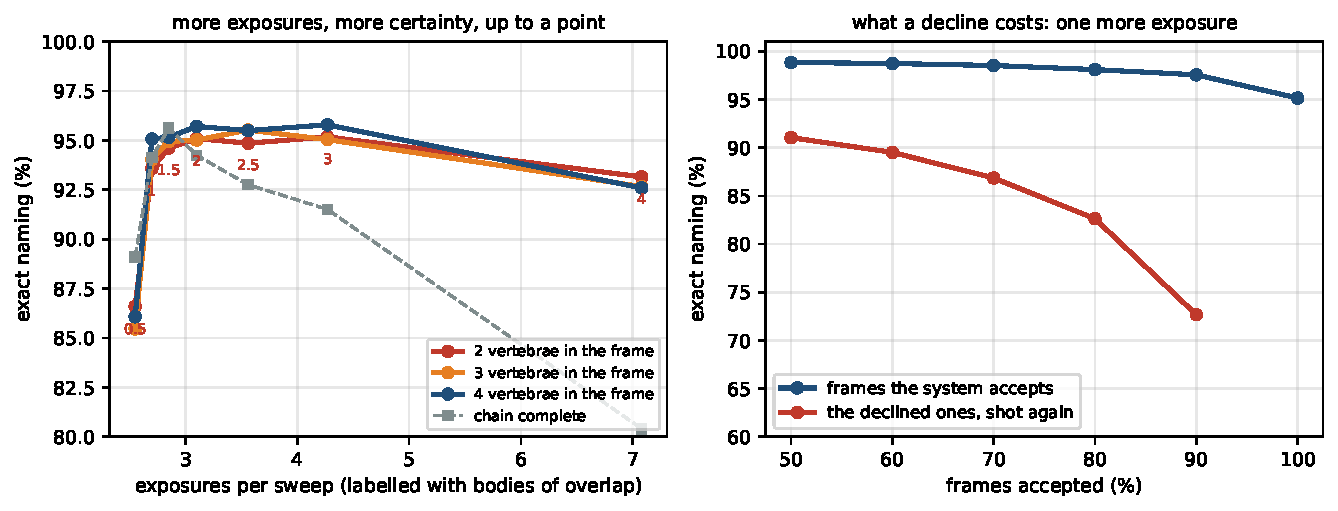
\includegraphics[width=\textwidth]{figures/fig15_spacing.pdf}
\caption{Left, exact naming and chain completeness against the number of exposures the sweep took, labelled with the overlap that produced them. Right, what a decline costs: the frames the system accepts against the same frames shot again.}
\end{figure}}{}

\subsection*{S1. Reproduction}
One job, \texttt{slurm/reproduce\_feasibility.sh}, recomputes every number from named inputs and writes \texttt{LEDGER.tsv} with the SHA-256 of each input and output per stage; \texttt{slurm/reproduce\_all.sh} chains the public downloads, renders, crop banks, encoder and head training, pseudolabelling, evaluation, and figure generation. \texttt{docs/FEASIBILITY\_REPRODUCE.md} names the origin of every input and the number each stage owns. Figures are drawn by \texttt{tools/make\_feasibility\_figures.py} from the stage JSONs; a missing stage renders a panel that says so.

\subsection*{S2. The report}
The feasibility analysis under test is reproduced in full as \texttt{Feasibility\_FOV.docx} in the repository so that every quotation can be checked against its source.

\subsection*{S3. CLAIM 2024}
The completed checklist accompanies the submission; items on data partitioning (patient-grouped, no film in both partitions), ground truth (label voxels for CT; dataset authors' reading for BUU; no reader of ours), model (architecture, loss, hyperparameters, seed, hash-recorded head--encoder pairing), evaluation (Wilson CIs on the vertebra; chance from the label distribution; film counts per stratum), and code and data availability are addressed in the Methods.

\subsection*{Table S1. How many vertebrae must be visible}
Exact naming in label-defined State C by window length $K$ (bank v2; Wilson 95\% CI on the vertebra; from \texttt{feasibility\_claims.json}, \texttt{by\_state\_and\_length\_C}). No real-film window longer than five exists, because the lumbar collections annotate L1--L5 only. The $K=5$ rows are whole annotated stacks whose names are fixed by the annotation convention and are NOT evidence of naming; the $K=2$--4 rows still include windows touching an end of the stack, whose crops show the unlabelled anchor. Pixel-defined interior results are in the text.

\begin{center}\small
\begin{tabular}{crrrr}\toprule
$K$ & Real film, anomalous & Real film, ordinary & Render, anomalous & Render, ordinary \\ \midrule
2 & 60.5 \ci{49.3}{70.8} (76) & 92.5 \ci{91.3}{93.5} (2,130) & 83.3 \ci{64.1}{93.3} (24) & 90.2 \ci{83.6}{94.3} (122) \\
3 & 82.9 \ci{74.8}{88.8} (111) & 95.6 \ci{94.8}{96.2} (3,156) & 88.2 \ci{76.6}{94.5} (51) & 98.0 \ci{94.3}{99.3} (150) \\
4 & 85.0 \ci{78.7}{89.7} (160) & 97.3 \ci{96.8}{97.8} (4,036) & 83.3 \ci{64.1}{93.3} (24) & 94.3 \ci{89.9}{96.9} (176) \\
5 & \textbf{100.0} \ci{98.3}{100.0} (225) & 100.0 \ci{99.9}{100.0} (5,170) & 88.0 \ci{76.2}{94.4} (50) & 96.7 \ci{92.4}{98.6} (150) \\ \midrule
\multicolumn{5}{l}{\emph{Bank v5 (30\% pseudolabelled crops), same evaluator}} \\
2 & 41.5 \ci{31.4}{52.3} (82) & 93.2 \ci{92.1}{94.2} (2,260) & 69.1 \ci{64.6}{73.2} (440) & 84.7 \ci{81.7}{87.3} (634) \\
3 & 61.8 \ci{53.0}{69.9} (123) & 95.5 \ci{94.7}{96.1} (3,354) & 76.3 \ci{72.7}{79.5} (615) & 86.3 \ci{83.6}{88.5} (750) \\
4 & 57.1 \ci{49.6}{64.4} (168) & 96.6 \ci{96.0}{97.1} (4,248) & 77.4 \ci{73.7}{80.7} (552) & 93.9 \ci{91.9}{95.4} (752) \\
5 & 85.1 \ci{80.0}{89.1} (235) & 99.6 \ci{99.4}{99.7} (5,335) & 90.6 \ci{87.8}{92.8} (530) & 98.2 \ci{96.9}{98.9} (705) \\ \midrule
\multicolumn{5}{l}{\emph{Bank v6 (no anomalous BUU film in training; anomalous CT renders $\times$4; all 144 anomalous studies in test), cross-entropy}} \\
2 & 68.5 \ci{64.7}{72.1} (606) & 93.2 \ci{92.0}{94.2} (2,104) & 88.9 \ci{74.7}{95.6} (36) & 90.0 \ci{83.3}{94.2} (120) \\
3 & 63.4 \ci{60.1}{66.6} (825) & 94.9 \ci{94.1}{95.6} (3,246) & 81.8 \ci{65.6}{91.4} (33) & 98.4 \ci{94.4}{99.6} (126) \\
4 & 78.4 \ci{75.8}{80.7} (1,100) & 98.0 \ci{97.5}{98.4} (3,948) & 89.3 \ci{72.8}{96.3} (28) & 97.1 \ci{92.9}{98.9} (140) \\
5 & 98.5 (1,495) \emph{whole stack} & 100.0 (5,195) \emph{whole stack} & 91.7 \ci{81.9}{96.4} (60) & 100.0 \ci{96.1}{100.0} (95) \\ \bottomrule
\end{tabular}
\end{center}


\end{document}
